\documentclass[journal]{IEEEtran}

\usepackage[utf8]{inputenc}
\usepackage[T1]{fontenc}
\usepackage{amsmath,amssymb,amsfonts}
\usepackage{graphicx}
\usepackage{booktabs}
\usepackage{array}
\usepackage{cite}
\usepackage{url}
\usepackage{balance}
\usepackage{xeCJK}
\setCJKmainfont{Heiti SC}

\graphicspath{{results/}}

\newtheorem{theorem}{定理}
\newtheorem{corollary}{推论}

\begin{document}

\title{面向预测式饱和管理的行为坐标实现接口\\[2pt]\large（中文译本）}

\author{Yongyan~Cao%
\thanks{预印本。本文已投稿，可能会用于发表；版权可能在不另行通知的情况下转让。}%
\thanks{Y.~Cao 就职于 Voryx Robotics LLC，San Jose, CA 95136, USA (e-mail: yongyancao@gmail.com)。本文为英文原稿的中文译本，内容以英文原稿为准。}%
}

\markboth{预印本}%
{Cao：面向预测式饱和管理的行为坐标实现接口}

\maketitle

\begin{abstract}
当机器人控制器请求的行为超出其执行器的实现能力时，力矩截断（clipping）能让下达给硬件的指令保持合法，但会改变实际被执行的行为。参考调节器（reference governor）、动作调节器（action governor）与预测安全滤波器已经确立了“对一个名义控制器进行监督”这一总体思路；本文所处理的是一个更狭窄的接口问题：如何在保留每个机器人各自随构型变化的力矩几何特性的同时，暴露出一个共同的任务加速度请求，并使“行为得以保留”这一说法背后的假设可被审计。名义的 PD、阻抗、训练策略、神经网络策略或条件化运动接口以 1~kHz 运行。一个 50~Hz 的 manager 将其请求的加速度通过一个机器人专属的实现模型进行映射，预测一个经不确定性收紧后的可行集，并在 QP 可行时返回一个最小代价的行为坐标修正量；一个最终投影作为快速执行器保护机制始终保留在环路中。一条单步引理把认证细化（certificate-refinement）的逻辑专门化到这一接口上，具体分解为三个条件：力矩预测精度、执行器裕度，以及行为后继失配；一条推论给出了双速率信号所额外需要的漂移界。这些是针对该接口的实现契约，而不是一个新的通用安全滤波器或认证迁移理论。在 111 组确定性降阶仿真运行中，全时域强制约束消除了仅约束第一步所遗留下来的一个预测中 3.587~Nm 的未来力矩违反。在确定性的留出（held-out）合成被控对象扰动下，一次采样式的起止点审计报告了三种实现映射下均为正的 T1、T2 松弛量，以及低于 0.03~m/s 预算的最大 $\ell_\infty$ T3 缺陷（均小于 0.0069~m/s）。一个时域匹配的轨迹参考调节器在成功案例中实现了相当的约束处理效果；所提出的向量修正方案在四个成功案例或时域隔离案例中的三个上具有更低的修正 RMSE，但并非在所有场景下都如此。突发扰动与严重的模型失配会违反两种预测式架构各自的审计前提。本研究在一个受控基准测试中，既展示又证伪了所提出的接口契约。
\end{abstract}

\begin{IEEEkeywords}
物理交互、执行器饱和、行为坐标接口、预测式约束管理、控制细化。
\end{IEEEkeywords}

\section{引言}
\label{sec:intro}

一个控制器计算出一个力矩请求 $\tau^0$，硬件实际施加的是
\[
\tau^{\mathrm{app}}
=
\operatorname{clip}\left(\tau^0,\ \tau_{\min},\ \tau_{\max}\right),
\]
也就是说，只要某个关节的力矩请求超出限制，就会被推回到最近的限制值。这个截断操作保护的是执行器，而不是行为本身。一旦截断被激活，机器人产生的加速度就不再是控制器所请求的加速度，因此机器人实际运行的也就不再是设计或训练时所依据的那个 PD、阻抗或学习到的控制律。而这一切在环路中不会有任何提示：控制器照常发出请求，执行器照常饱和，实际被实现的闭环动力学则悄无声息地偏离了预期。在物理交互场景中，这一点尤为关键，因为被请求的加速度正是决定表观柔顺性与扰动响应的关键量。

不同的控制器会通过不同的途径走到这一步。一个固定增益的 PD 律，是通过较大的跟踪误差走到这一步的。一个阻抗律 $M_d\ddot e=-K_de-D_d\dot e+F_h$，即便跟踪误差很小，也会通过接触力走到这一步。一个用 $\tanh$ 压缩输出的学习策略，其请求的\emph{加速度}是有界的，但该加速度所对应的力矩取决于当前构型，因此对请求本身设界并不等于对力矩设界。而一个上游的、由语言或扩散模型条件化生成的模块，甚至可能完全没有表征所执行机器人的执行器限制。途径各不相同，失效方式却是一样的。

保持名义控制器不变，但要求它暴露出一个任务加速度请求；再加入一个慢得多的层，用来预测每个机器人能否实现该请求，并以同样的行为坐标输出一个修正量。

\begin{quote}
\emph{名义控制器以其自身较高的伺服节拍不加改动地运行。一个慢得多的 manager 把它的行为请求沿一个短时域向前滚动预测，重建出当前执行机器人力矩可行的加速度集合，并在其 QP 可行时，在硬性截断被真正需要之前，对被请求的加速度施加一个最小代价的修正。}
\end{quote}

manager 既不选择任务，也不替代控制器。因为它的职责是预测与修正，而不是被动反应，所以它也不需要以伺服节拍运行；它究竟能运行得多慢，一般取决于所处的工作区域与所用模型（第~\ref{sec:experiments}节给出了一组具体的速率取值）。它唯一的职责，就是让请求在物理上可实现，同时尽可能贴近控制器原本的请求。一个最终的高速率投影仍然保留在环路中，用于应对在两次 manager 更新之间到来的扰动；预测与“最后一道防线”式的保护是两个相互独立的职责，第~\ref{sec:experiments}节表明它们可能在不同的时刻各自被需要。

一次性检查回答的是“这条指令现在合法吗？”这与“这个已规划的序列会一直保持合法吗？”并不是同一个问题。由于位置与速度会持续累积，一个未来才会出现的约束，可能要求提前改变当下的加速度，才能在到达限制那一步之前完成调整。这一区分在预测式约束管理中是标准做法 \cite{r3,r5,r16,r17,r18}。图~\ref{fig:horizon} 隔离出了它在本文所提接口中的作用：在时域斜坡场景中，约束每一个被预测的动作能消除计划中的力矩超限，而只约束第一步则会留下一个 3.587~Nm 的未来违反，以及 31.180~mm 的工作空间超限（第~\ref{sec:anticipatory}节）。

反馈线性化到一个类双积分器的行为模型是经典做法 \cite{r1,r2}。参考调节器、广义动作调节器、预测安全滤波器、抗积分饱和控制、模型预测式约束处理，以及任务空间容量多面体，都是已确立的方法 \cite{r3,r4,r5,r6,r7,r16,r17,r18,r19,r20}。本文并不主张拥有其中任何一项。双积分器、QP，以及射线到多面体的权限计算，都是实现所用的组成部件，而不是独立的贡献点。

我们真正提出的问题是：

\begin{quote}
能否在不隐藏机器人专属执行器几何特性的前提下，对一个共同的行为加速度请求进行监督，并能否把“行为保留”与“物理可实现性”之间的边界，表述为一组实现层面可审计的量？
\end{quote}

本文给出的回答是一种接口分解，而不是一类新的受约束控制器。行为动力学提供共享的请求坐标与认证坐标；力矩映射、可行集与不确定性界仍然是机器人专属的。第~\ref{sec:certificate}节把已有的细化逻辑 \cite{r8,r9,r19} 专门化为三个量，用来揭示这一特定的“加速度到力矩”接口在何时是可信的。

\textbf{贡献。}
\begin{enumerate}
\item 一种行为坐标实现接口：不同的名义控制器暴露出同一个任务加速度请求，而每个被执行的机器人则各自保留自己随构型变化的加速度到力矩映射与可行集。
\item 一种双速率实现方案：预测式地修正行为请求，在快速通道上重新计算机器人专属的实现映射，并报告标量力矩裕度与方向性加速度权限；这些组成部分是为保留该接口而被组装在一起的，而不是作为新的调节器、MPC 或多面体理论被提出的。
\item 把单步认证细化专门化到执行器实现上，分离出力矩预测精度（T1）、执行器裕度（T2）与行为后继失配（T3），并在 QP 中强制执行一个最小化的速度认证动作集。另一条独立的推论给出了双速率实现所需要的额外力矩漂移与平均请求条件。这些是可核查的接口条件，而不是一个通用的认证迁移定理。
\item 一项可复现的、包含 111 次运行的降阶研究，其中包括一个时域匹配的轨迹参考调节器对比、确定性的留出被控对象扰动、跨矩阵重复的锚点案例、五种控制器接口、三种实现映射、八种压力场景、T1--T3 审计，以及显式给出的负面案例（参数与完整制品见补充材料存档）。
\end{enumerate}

这些实验确立的是本接口的内部运行方式与失效检测能力。所实现的对比对象是一个在模型与计算预算上匹配的、ERG 风格的有限时域轨迹参考调节器，而不是对 \cite{r17} 中 Lyapunov/动态安全裕度构造的精确复现。因此，这些实验并不能确立“其他参考/动作调节器或预测安全滤波器不能实现同样的行为坐标”，也不能替代硬件验证。

\textbf{记号。} 全文统一使用下表符号。所有向量不等式均按分量（逐关节）成立。

\begin{table}[t]
\caption{记号}
\label{tab:notation}
\centering
\footnotesize
\setlength{\tabcolsep}{3pt}
\begin{tabular}{@{}p{1.7cm}p{5.3cm}p{0.7cm}@{}}
\toprule
符号 & 含义 & 单位 \\
\midrule
$\tau^0$ & 名义控制器请求的力矩 & Nm \\
$\tau^{\mathrm{pre}}$ & 在任何截断\emph{之前}本应被发送的力矩 & Nm \\
$\tau^{\mathrm{app}}$ & 截断之后实际施加的力矩 & Nm \\
$\hat\tau$ & manager 对 $\tau^{\mathrm{pre}}$ 的\emph{预测} & Nm \\
$\tau_{\min},\tau_{\max}$ & 执行器限制 & Nm \\
$\tau_{\mathrm{base}}$ & 已被占用的力矩：重力、科氏力、姿态、零空间 & Nm \\
$F_h$ & 测得的交互力 & N \\
$G_F(x)$ & 把 $F_h$ 转换为任务加速度单位；一般形式为 $\Lambda^{-1}(x)$，本基准测试使用 $\tfrac1m I$ & 1/kg \\
$a$ & 请求的任务加速度（决策变量） & m/s$^2$ \\
$a^{0}$ & 名义控制器请求的加速度 & m/s$^2$ \\
$\Delta a=a-a^{0}$ & manager 施加的修正量 & m/s$^2$ \\
$p,v$ & 任务位置与速度，直接向前传播 & m, m/s \\
$z=[p;v]$ & 任务状态 & --- \\
$e_c=p-p_r(t)$ & 控制器自身相对其参考 $p_r(t)$ 的跟踪误差；属于控制器内部量，不属于 $z$ & m \\
$\mathcal X$ & 作用于 $z$ 上的运行工作空间与速度盒约束 & --- \\
$H(x)$ & 把请求的加速度映射为其所需力矩 & Nm\,s$^2$/m \\
$\mathcal A(x)$ & 在当前构型下、通过 $H(x)$ 与 $\tau_{\mathrm{base}}(x)$ 判定为合法的、接口可实现的加速度集合 & m/s$^2$ \\
$\mathcal A^{\mathrm{tight}}(x)$ & 同一集合，经不确定性裕度收紧后的版本 & m/s$^2$ \\
$\bar\delta_\tau$ & 真实力矩与预测值之间可能的最大差距 & Nm \\
$\alpha^{+}$ & 给定方向上剩余的加速度权限 & m/s$^2$ \\
$\mathcal S_v=\{y:\|y\|_\infty\le v_{\max}\}$ & 已认证的速度区域 & --- \\
$\epsilon_v$ & 认证裕度：认证机制所能容忍的单步速度误差 & m/s \\
$\mathcal K_v(y)$ & 已认证动作集：从 $y$ 出发、在最多 $\epsilon_v$ 误差下仍停留在 $\mathcal S_v$ 内的请求集合 & m/s$^2$ \\
\bottomrule
\end{tabular}
\end{table}

有两个集合运算仅出现在第~\ref{sec:certificate}节，二者都有直白的含义：$\mathcal X\oplus\mathcal Y$ 表示“$\mathcal X$ 中任意一点加上 $\mathcal Y$ 中任意一点”（对两者取最坏情形），$\mathcal X\subseteq\mathcal Y$ 表示“$\mathcal X$ 完全落在 $\mathcal Y$ 之内”。

\section{方法的工作方式}
\label{sec:howitworks}

本节先把整个回路完整地过一遍，之后再对其进行形式化。

\textbf{快循环，以控制器自身较高的伺服节拍 $T_f$ 运行，与当前使用哪个控制器无关。} 先求值名义控制器，得到其请求的加速度 $a^0$，通过实现映射（第~\ref{sec:realizable}节）转换为力矩 $\tau^0$。加上 manager 最近一次发布的修正量，按\emph{当前}构型转换为力矩：
\[
\tau^{\mathrm{pre}}=\underbrace{\tau^0}_{\text{控制器}}+\underbrace{H(x)\,\Delta a}_{\text{manager 的修正}},
\]
然后施加最终的高速率投影，即最后一道防线，
\[
\tau^{\mathrm{app}}=\operatorname{clip}\left(\tau^{\mathrm{pre}},\ \tau_{\min},\ \tau_{\max}\right),
\]
这就是最终发送给机器人的量。

\textbf{慢循环，每个 manager 周期 $\Delta t$ 运行一次，远长于 $T_f$。} manager 发布的修正量是\emph{加速度}形式，而不是缓存的力矩；$H(x)$ 在每一个快循环节拍都会被重新计算，因此两次 manager 更新之间的构型漂移，不会把一个已过期的方案变成一个人为制造出来的扰动。每次更新执行以下步骤：
\begin{enumerate}
\item 把名义控制器向前滚动 $N=12$ 步，得到请求的加速度序列 $a^0_0,\dots,a^0_{N-1}$ 以及预测状态。
\item 在每个预测状态上，构建该机器人实际可实现的加速度集合，并按不确定性裕度收紧。
\item 求解一个小型 QP，在满足上述集合、工作空间盒约束，以及第~\ref{sec:certificate}节速度认证集合的前提下，找到与名义请求最接近的加速度序列。
\item 发布第一步的修正量 $\Delta a$；记录裕度与方向性权限。
\end{enumerate}

如果名义滚动预测本身已在各处都可行，QP 会原样返回名义请求，修正量为零——在正常运行时，manager 处于未激活状态。

\textbf{预见机制体现在何处。} 这里并不存在一个独立的“饱和检测器”。沿着名义滚动预测，预测力矩为 $\hat\tau=\tau_{\mathrm{base}}+H(a^{0}-G_F\hat F_h)$；一旦该力矩在时域中的任意一步进入被收紧的边界层，相应的约束就会被激活，QP 就会被迫做出调整。这个收紧机制正是让约束能够\emph{提前}生效的原因；而位置与速度的前向传播，则是把一个“未来才会激活”的约束，转化为一个“当下就需要处理”的修正的原因。

\section{相关工作与定位}
\label{sec:related}

阻抗控制指定了一个期望的运动-力关系 \cite{r1}，操作空间控制则把任务加速度或力旋量映射为关节力矩 \cite{r2}。两者都依赖于充足的执行器权限。抗积分饱和方法处理的是某一特定闭环内部由饱和引发的性能退化 \cite{r6,r7}，而模型参考自适应阻抗控制则试图在动力学不确定的情况下复现目标阻抗 \cite{r11}。交互控制类 MPC 方法则转而利用学习到的交互动力学、高斯过程或环境估计，自适应地调整阻抗参数或轨迹 \cite{r12,r13,r14,r15}。本文并不替代这些控制器：它要求上游控制器暴露一个任务加速度请求，并监督某个机器人能否实现该请求。

参考与指令调节器是已确立的附加机制，通过修改参考量，使一个已预先稳定的系统保持在约束内 \cite{r3}。Ambrosino 等人直接针对机器人执行器饱和问题，提出了一种基于轨迹的显式参考调节器，保留了内部 PD 控制器，并在一台七自由度 KUKA 机械臂上验证了位置、速度与饱和处理效果 \cite{r17}。广义动作调节器把监督器放在控制器之后，修改的是动作而不是参考量，并通过有界不确定性下的安全可返回集合，提供全时段的约束保证 \cite{r18}。预测安全滤波器同样接受一个名义动作，使用一个预测模型与不确定性描述，并对不安全动作进行最小化替换；其终端安全策略支持一种本文并不具备的递归保证 \cite{r5,r16}。因此，保留控制器、预测约束，以及最小化动作修改，都属于已有工作。本文更狭窄的设计选择在于\emph{动作表示方式}：不同的控制器暴露出任务加速度，而一个独立的实现对象则把它映射为随构型变化的机器人力矩，并暴露出 T1--T3 审计量。

机器人能力与加速度多面体，早已把关节力矩盒约束映射为任务空间力或加速度集合，射线到边界的计算也早已能够量化方向性容量 \cite{r20}。本文利用这些思路来构建 $\mathcal A(x)$ 与 $\alpha^+$，并不是提出新的多面体理论，而是将其作为行为-实现接口中机器人专属的那一半。

认证论证同样建立在近似仿真、细化与基于契约的设计之上 \cite{r8,r9,r10}。近期关于控制屏障函数迁移的工作，利用仿真函数与显式裕度，把一个认证从双积分器迁移到完整的非线性四旋翼动力学，并用一个 QP 滤波器加以强制执行 \cite{r19}。那个框架更为通用，并提供了一个实质性的连续时间迁移构造。第~\ref{sec:certificate}节则转而给出一个刻意保持基础性的、面向执行器实现的离散单步专门化：T1 与 T2 分离出的是“一个被预测的行为请求能否在不被截断的情况下通过力矩接口”，T3 分离出的是“其物理后继是否落在行为认证的误差预算之内”。

面向接触的调节器进一步展示了模块化约束管理架构的丰富程度。Gautam 等人提出的柔顺 ERG，在规划器与控制器之间插入一个参考管理器，并使用一个能量认证来实现对接触友好的操作，同时给出了硬件验证 \cite{r21}。它在被监督的量与认证机制上都有所不同，但也进一步说明了为何本文的主张必须针对一个具体的接口与审计分解，而不是“存在某种附加安全层”这一泛泛的说法。

\begin{table*}[t]
\caption{与最接近的方法族之间的定位对比}
\label{tab:positioning}
\centering
\footnotesize
\setlength{\tabcolsep}{4pt}
\begin{tabular}{@{}p{3.0cm}p{2.6cm}p{4.6cm}p{5.6cm}@{}}
\toprule
方法 & 被监督的量 & 主要保证或证据 & 与本文的区别 \\
\midrule
饱和感知轨迹 ERG \cite{r17} & 关节参考量 & 已预测的关节/速度约束，并在 KUKA 硬件上验证 & 使用一条 PD 专属的参考通道；不具备通用的行为加速度/实现审计 \\
预测安全滤波器 \cite{r16} & 被控对象输入/动作 & 具不确定性感知的预测式滤波，配有终端安全策略 & 更为通用且具有递归基础；未分离出加速度到力矩的 T1--T3 接口 \\
广义动作调节器 \cite{r18} & 控制器之后的动作 & 具安全可返回集合保证的状态/输入约束 & 通用的动作监督；不含机器人任务加速度实现对象 \\
任务空间容量多面体 \cite{r20} & 能力集合，而非一个监督器 & 实时的力/速度/加速度容量计算 & 提供了本文所用的几何工具，但不含双速率修正或接口契约 \\
迁移型 CBF \cite{r19} & 具体系统安全滤波器的输入 & 基于仿真函数、向非线性动力学迁移的认证 & 通用的连续时间迁移理论；未针对截断与力矩可实现性做专门化 \\
柔顺 ERG \cite{r21} & 运动参考量 & 具仿真与硬件证据的接触能量认证 & 参考量与能量接口，而非行为加速度与 T1--T3 \\
本文 & 任务加速度请求 & 有限时域 QP 加一个采样式单步实现审计 & 显式的行为请求/机器人实现分离；不具备递归或硬件层面的保证 \\
\bottomrule
\end{tabular}
\\[2pt]
\raggedright\footnotesize 表 I. 与最接近的方法族之间的定位对比。该对比是架构与定理层面的。第~\ref{sec:experiments}节还额外实现了一个与本基准测试匹配的、ERG 风格的时域轨迹参考调节器；它并不是对 \cite{r17} 的精确复现。
\end{table*}

\section{对某个给定机器人而言，“可实现”意味着什么}
\label{sec:realizable}

对于一个力矩控制的机器人，
\[
M(q)\ddot q+h(q,\dot q)=\tau+J(q)^\top F_h,
\]
其中 $M(q)\succ0$，$h$ 是建模出的重力/科氏力/摩擦项，$F_h$ 是测得的交互力（本基准测试中是一个二维向量，而不是完整的力旋量）。执行器限制是盒约束 $\tau_{\min}\le\tau\le\tau_{\max}$。

本架构对名义控制器只提出三点要求：其\textbf{当前请求的任务加速度} $a^0$；一项可选的\textbf{预见（preview）}能力，即能够沿一条预测轨迹被求值；以及一个\textbf{关于该预见可能有多不准的界}。一个解析形式的 PD 或阻抗律可以直接沿预测状态求值。一个学习得到的策略可以在预测观测上被查询。如果不存在经过验证的预见方式，可以使用零阶保持或一个学习到的预测器，但由此产生的误差必须被纳入该界之中。一个既没有查询接口、也没有有界预见误差的黑箱控制器，不在本认证的适用范围之内。诱导出的力矩 $\tau^0$ 是通过下文的实现映射，由 $a^0$ 得到的。

用任务状态 $z=[p;v]$——绝对的任务位置与速度，直接向前传播，而不是相对于一个可能随时间变化的参考——来表示，局部工作区域内被请求的行为为
\[
\ddot p=a+d_{\mathrm{res}},
\]
\emph{文字说明：} 任务实际实现的加速度，等于请求加速度加上一个残余扰动 $d_{\mathrm{res}}$。一旦引入下文式\eqref{eq:iv0}的交互力补偿，$d_{\mathrm{res}}$ 就不再包含 $F_h$ 自身（已被补偿的）那部分贡献，而只包含该补偿未能覆盖的部分——残余的力模型误差、交叉耦合、离散化误差——第~\ref{sec:certificate}节把它显式地作为一个单步模型误差加以核查。一个参考跟踪型控制器，可以另外形成其自身相对参考 $p_r(t)$ 的跟踪误差 $e_c=p-p_r(t)$ 来计算其请求；这一控制器内部误差本身并不属于 $z$ 的一部分。

在一个 manager 周期内对其积分，得到恒加速度更新式
\[
p^{+}=p+\Delta t\,v+\tfrac12(\Delta t)^2(a+d_{\mathrm{res}}),
\qquad
v^{+}=v+\Delta t\,(a+d_{\mathrm{res}}),
\]
这就是标准的 $z^{+}=Az+B(a+d_{\mathrm{res}})$ 双积分器。它是一个共享接口，而不是被主张的新颖之处。

要实现一个请求的加速度 $a$，是要付出力矩代价的。对于完整刚体模型，令 $N_\tau(q)\tau_{\mathrm{sec}}$ 表示满足 $JM^{-1}N_\tau=0$ 的、动力学一致的次级力矩。操作空间实现所需要的偏置与次级贡献为
\begin{align}
\tau_{\mathrm{base}}(x)
&=J^\top\Lambda\bigl(JM^{-1}h-\dot J\dot q\bigr)
+N_\tau\tau_{\mathrm{sec}}, \nonumber\\
H(x)&=J(q)^\top\Lambda(q),
\quad
\Lambda=\left(JM^{-1}J^\top\right)^{-1},
\quad
G_F(x)=\Lambda^{-1}(x).
\label{eq:iv0}
\end{align}
指令力矩为
\begin{equation}
\tau=\tau_{\mathrm{base}}(x)+H(x)\,\bigl(a-G_F(x)F_h\bigr).
\label{eq:iv0a}
\end{equation}

代入机器人动力学可得 $\ddot p=a$：$JM^{-1}h$ 与 $\dot J\dot q$ 两项相互抵消，动力学一致的次级力矩不进入任务加速度，而 $HG_FF_h=J^\top F_h$ 抵消了被建模的交互力项。因此，$a$ 是期望的\emph{总}任务加速度，而不是相对某个独立扰动项定义出来的残差。这一结论仍以所给出的偏置表达式与动力学一致性为前提。任何被遗漏的摩擦、不完美的偏置项、未解耦的次级力矩，或力模型误差，都应归入 $d_{\mathrm{res}}$、$\bar\delta_\tau$，或单步失配界，而不应被该恒等式悄悄地吸收掉。第~\ref{sec:experiments}节的降阶基准测试并不主张这一完整推导：它直接实例化 $\tau_{\mathrm{base}}$ 与 $H$，并使用标量近似 $G_F=\tfrac1m I$（有效任务空间质量 $m$，见附录~\ref{app:params}），仅在 $\Lambda\approx mI$ 时精确成立。

我们假设在整个已验证的工作区域内，$J(q)$ 始终保持行满秩，且 $JM^{-1}J^\top$ 在该区域内均匀非奇异，即 $\lambda_{\min}(JM^{-1}J^\top)\ge\underline\lambda>0$；不满足这一条件的构型不在本认证的适用范围之内。在这类构型附近，实现中可以使用一个阻尼化的操作空间逆，但由此产生的加速度实现缺陷，必须被纳入 $\bar\delta_\tau$（力矩域）或单步模型误差界（速度域），而不能被假设为不存在。

\emph{文字说明：} $H(x)$ 是在当前构型下、在式\eqref{eq:iv0}的力补偿之后，每单位净任务加速度所需付出的关节力矩代价。只有当这一代价落在剩余预算之内时，一个请求才是可实现的：
\begin{equation}
\tau_{\min}\ \le\ \tau_{\mathrm{base}}(x)+H(x)\,(a-G_F(x)F_h)\ \le\ \tau_{\max}.
\label{eq:iv1}
\end{equation}

把满足式\eqref{eq:iv1}的 $a$ 构成的集合称为\textbf{可行请求集} $\mathcal A(x)$。这个对象无法被做成与机器人无关的：它会通过 $H(x)$ 与 $\tau_{\mathrm{base}}(x)$ 随构型一起移动，而去掉这种依赖关系，恰恰就会去掉引发饱和的那部分几何特性。

\textbf{接口一致性。} 名义接口提供一个请求的任务加速度 $a^0$，要么如第~\ref{sec:experiments}节中每个被评测的控制器那样直接给出，要么对于一个不透明的、只输出力矩的控制器，通过一个满足下述残差界的机器人专属转换给出。由此诱导出的名义力矩为
\[
\tau^0=\tau_{\mathrm{base}}(x)+H(x)(a^0-G_F(x)F_h)+r_\tau(x),
\qquad
|r_\tau(x)|\le\bar r_\tau,
\]
其中 $r_\tau$ 是一个接口一致性残差，被下文的收紧裕度 $\bar\delta_\tau$ 所约束；第~\ref{sec:experiments}节所评测的五种接口在构造上均满足 $r_\tau\equiv0$。

条件~\eqref{eq:iv1}在 $a$ 空间中是一组平行的板状约束，每个关节一对，因此 $\mathcal A(x)$ 本身在加速度空间中已经是一个多面体。

由此产生两个在后文会被用到的实际后果。
\begin{itemize}
\item \textbf{它不是一个球。} 权限是方向相关的。机器人整体上可能仍有充裕的剩余力矩，却几乎无法沿某一个特定方向加速。
\item \textbf{探测它的代价很低。} 方向性权限可以直接从第~\ref{sec:reports}节所定义的 $\mathcal A^{\mathrm{tight}}(x)$ 的半空间表示中求得，不需要枚举顶点。
\end{itemize}

manager 预测的是 $\hat\tau$；而实际会被发送的力矩 $\tau^{\mathrm{pre}}$ 与之存在差异。假设这一差异逐关节有界：
\begin{equation}
\left|\tau^{\mathrm{pre}}-\hat\tau\right|\ \le\ \bar\delta_\tau.
\label{eq:iv2}
\end{equation}

那么仅仅让\emph{预测值}落在盒约束内是不够的；预测值加上其误差也必须落在盒约束内。因此 manager 强制执行以下\textbf{收紧后}的条件：
\begin{equation}
\tau_{\min}+\bar\delta_\tau\ \le\ \hat\tau\ \le\ \tau_{\max}-\bar\delta_\tau,
\label{eq:iv3}
\end{equation}
我们用 $\mathcal A^{\mathrm{tight}}(x)$ 表示满足该条件的加速度集合。式~\eqref{eq:iv3}就是整个收紧机制：在每个执行器限制内侧留出一个宽度为 $\bar\delta_\tau$ 的边界层。正是它使约束能够在到达物理极限\emph{之前}而不是恰好在极限处生效，第~\ref{sec:ablation}节展示了去掉它之后会发生什么。

界 $\bar\delta_\tau$ 必须覆盖状态估计误差、两次 manager 更新之间的插值、次级力矩、力矩变化率限制（若存在——本实现中不存在），以及其他任何可能改变截断前力矩的实现效应。本实现使用它的两种具体实例：一种是保守的、与动作无关的 $\bar\delta_\tau^{\mathrm{QP}}$，在 QP 自身的收紧约束中，按加速度极限（而不是尚未被选定的请求）求值；另一种是较小的、与动作相关的 $\bar\delta_\tau(a,F_h)$，在第~\ref{sec:experiments}节的 (T1) 审计中，按实际求解得到的请求求值。由于 QP 的界是在最坏情形加速度处求值的，在整个加速度盒约束范围内都有 $\bar\delta_\tau^{\mathrm{QP}}\ge\bar\delta_\tau(a,F_h)$。

\textbf{问题表述。} 给定一个提供 $a^{0}$ 的名义控制器，寻找一个修正量 $\Delta a$，使得：
\begin{enumerate}
\item $a=a^{0}+\Delta a$ 与名义请求保持接近；
\item 考虑到不确定性，已实现的力矩在整个时域内都落在执行器盒约束之内；
\item 预测状态满足运行中的工作空间与速度约束；并且
\item 该结果能够针对“把一个独立确立的行为认证进行迁移”所需的充分条件进行检验。
\end{enumerate}

\section{预测式修正与 manager 所报告的内容}
\label{sec:correction}

\subsection{预测式修正}
\label{sec:predictivecorrection}

名义控制器与映射 $H(x)$ 每个快循环周期 $T_f$ 都会被求值，最终的力矩盒投影也是如此；manager——包括下文引入的、对相邻已规划步的速率约束，该约束仅在 QP 被求解时才会被求值——则每个 manager 周期 $\Delta t$ 运行一次，远长于 $T_f$。在一次 manager 更新内，我们用 $a_i$ 表示时域第 $i=0,\dots,N-1$ 步的请求，用 $a^0_i$ 表示名义控制器在该处本会请求的值；由于下文的一切都发生在单次更新内部，因此省略了 manager 更新的索引。在 $i=0$ 处，$a_{-1}$ 指的是 manager 自己在\emph{上一次}更新\emph{开始}时所求解出的 $a_0$，而不是那次更新未经修正的名义值，因此下文的速率约束与平滑项，约束的是相对于 manager 自身上一次决策的变化。

决策变量是\emph{完整}的请求 $a_i$，而不是修正量本身——约束是作用在实际请求上的物理条件，修正量是事后读出的。对每个 $i$ 分别满足：一个预测行、一个可实现性行、一个速度认证行、一个工作空间行，以及一个请求速率行：
\small
\begin{align}
\min_{a_0,\dots,a_{N-1}}\quad
&\sum_{i=0}^{N-1}
\Big(
\underbrace{\|a_i-a^0_i\|^2_{W}}_{\text{贴近控制器}}
+\underbrace{\|a_i-a_{i-1}\|^2_{W_\Delta}}_{\text{保持平滑}}
\Big)\nonumber\\[2pt]
& p_{i+1}=p_i+\Delta t\,v_i+\tfrac12(\Delta t)^2a_i,
\quad v_{i+1}=v_i+\Delta t\,a_i, \nonumber\\
& \tau_{\min}+\bar\delta_{\tau,i}^{\mathrm{QP}}\le\tau_{\mathrm{base}}(\hat x_i)+H(\hat x_i)\,(a_i-G_F(\hat x_i)\hat F_{h,i}) \nonumber\\
&\hspace{4.7em}\le\tau_{\max}-\bar\delta_{\tau,i}^{\mathrm{QP}}, \nonumber\\
& |v_i+\Delta t\,a_i|\le v_{\max}-\epsilon_v,
\quad z_{i+1}\in\mathcal X, \nonumber\\
& \|a_i\|_\infty\le a_{\max},
\quad
\|a_i-a_{i-1}\|_\infty\le\dot a_{\max}\Delta t.
\label{eq:qp}
\end{align}
\normalsize

每一条约束在 $a_i$ 中都是线性的，目标函数是凸二次的，因此这是一个小型稠密 QP。这里 $\hat x_i$ 是用于组装该 QP 的固定名义滚动预测上的状态，$\hat F_{h,i}$ 是时域第 $i$ 步的预测交互力——默认情况下是把测得的力在整个时域上保持不变（一种零阶保持；第~\ref{sec:anticipatory}节的预见失配案例正是这一选择所对应的失效模式），第~\ref{sec:ablation}节的消融实验中还评测了其他预见策略——而 $\mathcal X=\{z:|p|\le\mathrm{pos}_{\max},\,|v|\le v_{\max}\}$ 是作用在任务状态 $z=[p;v]$ 上的运行工作空间与速度盒约束。速度认证这一行，写出来就是第~\ref{sec:certificate}节的集合 $\mathcal K_v$：它把 $\mathcal X$ 内部原本对预测速度的普通约束 $v_{\max}$，在向前一个 manager 步的范围内，替换为更紧的 $v_{\max}-\epsilon_v$。连同可实现性这一行，一个可行解在构造上就满足 $a_i\in\mathcal A^{\mathrm{tight}}(\hat x_i)\cap\mathcal K_v(v_i)$——这正是定理~\ref{thm:transfer}前提中“已认证动作集”与“已收紧执行器”这两部分，而不是事后才附加上去的检查。状态、加速度、认证与速率方面的约束全部是硬约束；不存在松弛变量，也没有另行构造终端不变集。

发布出去的修正量是第一步的差值：
\[
\Delta a=a_0-a^0_0.
\]

\textbf{解读。} manager 首先针对以上每一条约束检查名义滚动预测；如果它已经全部满足，就原样返回该滚动预测，$\Delta a=0$。否则求解该 QP，返回代价最小的调整量——同时对偏离名义行为与整个时域内修正请求的变化进行惩罚——把请求拉回到可行集的边界上。

该 QP 是沿着\emph{被冻结的名义滚动预测}组装的，这使得每一条可实现性约束都保持线性；如果该滚动预测是错的——无论是由于预见失配，还是因为 QP 自身的修正把轨迹带离了名义轨迹——当前计划所依据的未来几何信息就可能变得不准确。本基准测试并未给出这种时域几何漂移的解析界——$\bar\delta_\tau$ 与条件 (T1) 约束的是在当前状态下求值的实现映射与模型不确定性（第~\ref{sec:sampled}节），是一个相关但不同的误差来源。频繁的重新规划限制了任何一个时域的几何信息被信任的时长，而模型失配与预见失配这两个案例，则从经验上展示了时域几何漂移的后果（第~\ref{sec:anticipatory}节）。

如果求解器报告不可行，实现会转而把第一个名义加速度，投影到当前被收紧的力矩与状态半空间上（这是一个连续时间的控制屏障函数集合，而不是 QP 自身的离散约束），并把这一反应式指令平铺到已存储的序列上，若连这一投影也为空则返回零加速度；无论哪种情形，最终的高速率投影都始终保持激活。这一后备方案给出一个确定性的有界指令，但\textbf{不能}恢复时域可行性，也不满足迁移条件——包含后备步骤的轨迹并不属于时域 MPC 行为。

\subsection{manager 所报告的内容}
\label{sec:reports}

对每个关节，报告尚未被使用的原始力矩裕度；所报告的裕度取各关节中最差的一个：
\[
\mu=\min_j\left\{\tau_{\max,j}-\tau_j,\ \tau_j-\tau_{\min,j}\right\}.
\]
因此 $\mu>0$ 表示每个关节都严格落在其限制内部，$\mu=0$ 表示某个关节恰好处于限制边界，$\mu<0$ 表示该请求不可实现。本基准测试使用对称限制，$\tau_{\min,j}=-L_j$、$\tau_{\max,j}=L_j$，因此该式化简为 $\min_j(L_j-|\tau_j|)$。$\mu$ 以牛顿·米为单位报告，并未按各关节自身的量程做归一化——一个力矩量程更宽的关节，其原始裕度本身就更大，因此 $\mu$ 在具有不同执行器限制的机器人之间不可直接比较。在整个时域上，我们报告其中的最小值。

标量裕度并不能揭示机器人是否仍能\emph{沿它所需要的方向}加速。给定一个\emph{可行}的当前加速度 $a_c\in\mathcal A^{\mathrm{tight}}(x)$ 与一个单位方向 $y$，沿 $y$ 方向剩余的权限，是在离开被收紧的可行集之前还能移动多远，因此该指标所计入的，正是优化器本身已经在强制执行的那同一个不确定性裕度：
\[
\alpha^{+}(x,a_c,y)=\max\left\{\alpha\ge0:\ a_c+\alpha y\in\mathcal A^{\mathrm{tight}}(x)\right\}.
\]

$\mathcal A^{\mathrm{tight}}(x)$ 是一个由每个执行器一条收紧板状约束所定义的多面体，$\{a:l_j\le h_j(x)^\top a\le u_j\}$，其中 $h_j(x)^\top$ 是 $H(x)$ 的第 $j$ 行；它本身未必是一个盒约束的仿射像，但这对 $\alpha^+$ 并不构成障碍：它仍然是一个闭式求值，而不是一次搜索，可以直接从 $\mathcal A^{\mathrm{tight}}(x)$ 的半空间形式 $\{v:Av\le b\}$（任何以这种形式表示的多面体都具备）得到：$\alpha^{+}=\min_{j:(Ay)_j>0}(b_j-(Aa_c)_j)/(Ay)_j$，即从 $a_c$ 出发、沿 $y$ 方向的射线首次离开该集合的位置。如果当前请求已经落在 $\mathcal A^{\mathrm{tight}}(x)$ 之外，manager 按约定报告 $\alpha^{+}=0$，而不再套用这一公式，因为该公式仅在从一个可行起点出发时才有意义。一个很小的 $\alpha^{+}$ 意味着\textbf{方向性权限崩溃}：机器人整体上可能仍保有充裕的未使用力矩，却仍然无法抵抗沿 $y$ 方向的一次推力。这正是单一利用率数字所掩盖的失效模式。

manager 还会报告其时域问题是否可行。这是一个有用的可恢复性指标，但\textbf{不是}隶属于某个已认证可行核（viability kernel）的证明，因为本文并未构造终端不变集或后备策略。因此第~\ref{sec:experiments}节使用“近边界制动压力案例”这一术语，而不是“不可挽回点”。

\section{一份有条件的实现契约}
\label{sec:certificate}

第~\ref{sec:realizable}--\ref{sec:certificate}节描述的是单个机器人。本节要问的是：当机器人发生变化时，什么东西是可以保留下来的。本节并不提出一个通用的认证迁移框架；它把细化逻辑专门化到加速度到力矩这一接口上，并精确指出对于一次迁移，哪些实现层面的量必须成立。

\subsection{用文字描述的问题设定}

假设已经有人证明了某个关于\emph{行为}的结论——例如，只要每一步的请求都来自某个\emph{可接受}的动作集合，而不是一个固定的策略，并且单步模型误差保持在裕度 $\epsilon_v$ 之内，那么速度就永远不会离开某个集合 $\mathcal S_v$。把这个结论称为\textbf{认证}。它不涉及任何具体机器人，而且它刻意不指定唯一的控制律：不同的机器人，或同一个机器人在不同时刻，可能需要从这个可接受集合中选取不同的成员，这并不是该认证的缺陷——恰恰相反，正因如此，真正可复用的对象是这个集合本身，而不是建立在它之上的任何一个具体策略。

现在把一个真实机器人放到这个认证之下。可能出错的地方有三处：
\begin{enumerate}
\item manager 的力矩预测 $\hat\tau$ 可能是错的；
\item 由此产生的力矩可能装不进执行器盒约束，于是截断被激活，机器人不再执行被请求的动作；
\item 即便没有发生截断，真实机器人的单步速度也可能与双积分器的预测相差超过认证所能容忍的范围。
\end{enumerate}

定理~\ref{thm:transfer}记录了由此产生的接口契约：针对 manager 从可接受集合中实际选出的任何请求，把上述三种情况都排除掉，单步认证的结论就随之成立。

\subsection{已认证动作集，以及为何只针对速度}

令 $y=v$ 为任务速度，$F_v(y,a)=y+\Delta t\,a$ 为其单步更新式（即第~\ref{sec:realizable}节双积分器中速度那一半）。定义已认证区域，其中裕度 $\epsilon_v$ 满足 $0<\epsilon_v<v_{\max}$，
\[
\mathcal S_v=\{y:\|y\|_\infty\le v_{\max}\},
\qquad
\mathcal E_v=\{d:\|d\|_\infty\le\epsilon_v\},
\]
并在每个 $y\in\mathcal S_v$ 处，定义\textbf{已认证动作集}
\[
\mathcal K_v(y)=\left\{a:\|F_v(y,a)\|_\infty\le v_{\max}-\epsilon_v\right\}.
\]

\emph{文字说明：} $\mathcal K_v(y)$ 是所有能够让下一步速度、在吸收了最多 $\epsilon_v$ 大小的单步模型误差之后，仍然落在已认证区域内的请求。位置被刻意排除在该认证之外——它仍然只是 $\mathcal X$ 中的一条普通运行约束——因为速度是本基准测试唯一真正测量并审计其单步失配的量（第~\ref{sec:sampled}节）；如果同时收紧位置约束，就没有相应的测量量来支撑它。

只要 $\epsilon_v/\Delta t$ 落在抽象模型可接受的加速度范围之内，$\mathcal K_v$ 在 $\mathcal S_v$ 上就永远不为空：以该速率减速，能在一个 manager 周期内消耗掉 $\epsilon_v$ 的速度，因此总是存在一个合法的请求，能把速度带回到更紧的区间内，即便有若干个速度分量同时处于边界上也是如此（附录~\ref{app:params}给出了这相对于本基准测试自身加速度界所留出的裕度）。这只是 $\mathcal K_v(y)$ 在抽象速度模型中单独的非空性；它与机器人专属的、被收紧的力矩集合 $\mathcal A^{\mathrm{tight}}(x)$，以及速率与状态约束的交集，仍然可能为空——第~\ref{sec:predictivecorrection}节的反应式后备方案存在的意义正是为了处理这种情况，第~\ref{sec:experiments}节的实验中也确实出现过这种情形。

\subsection{单步接口引理}

记 $\Pi(x)=y=v$ 为从物理状态到该认证所表述的任务速度之间的映射，令 $f^d(x,\tau,F_h)$ 表示单步物理动力学：即从状态 $x$ 出发，在力 $F_h$ 下施加力矩 $\tau$ 之后，一个 manager 周期之后机器人实际到达的状态。

\begin{theorem}[单步条件式速度认证实现]
\label{thm:transfer}
假设物理状态 $x$ 落在一个已验证的工作区域内，$\Pi(x)\in\mathcal S_v$，且请求 $a$ 满足 $a\in\mathcal K_v(\Pi(x))$——是这样的任意 $a$，而不是某一个特定的策略。若：

\textbf{(T1) 预测精度。} 本应被发送的力矩落在 manager 预测值所声明的界内，
\[
\left|\tau^{\mathrm{pre}}-\hat\tau\right|\le\bar\delta_\tau.
\]

\textbf{(T2) 执行器裕度检验。} 经该界放宽之后的预测值，仍然落在执行器盒约束之内，
\[
\tau_{\min}+\bar\delta_\tau\ \le\ \hat\tau\ \le\ \tau_{\max}-\bar\delta_\tau .
\]

\textbf{(T3) 认证裕度检验。} 真实机器人与双积分器预测之间的单步速度失配，落在认证裕度之内，
\[
\left\|\Pi\!\left(f^d(x,\tau^{\mathrm{pre}},F_h)\right)-F_v\!\left(\Pi(x),a\right)\right\|_\infty\ \le\ \epsilon_v .
\]

那么截断不会改变 $f^d$ 中所代表的、被冻结的力矩输入，$\tau^{\mathrm{app}}=\tau^{\mathrm{pre}}$，且相应的物理后继状态仍停留在已认证区域内，
\[
\Pi\!\left(f^d(x,\tau^{\mathrm{app}},F_h)\right)\in\mathcal S_v .
\]
\end{theorem}

\begin{IEEEproof}
(T1)+(T2) 给出 $\tau_{\min}\le\tau^{\mathrm{pre}}\le\tau_{\max}$，因此截断未被激活，$\tau^{\mathrm{app}}=\tau^{\mathrm{pre}}$。
(T3) 把真实的单步后继状态置于 $F_v(\Pi(x),a)\oplus\mathcal E_v$ 之内。
根据 $\mathcal K_v$ 的定义，该集合本身就落在 $\mathcal S_v$ 之内。
\end{IEEEproof}

\begin{corollary}[条件式双速率区间实现]
\label{cor:tworate}
令第 $k$ 次 manager 更新覆盖区间 $[t_k,t_{k+1}]$，令 $a_f(t)$ 为在保持 $\Delta a_k$ 不变的同时、重新求值名义控制器所产生的时变快循环请求。定义其区间平均
\[
\bar a_k=\frac{1}{\Delta t}\int_{t_k}^{t_{k+1}}a_f(t)\,dt
\]
（在实现中对应于二十个 1~kHz 采样点的相应平均）。假设 $\bar a_k\in\mathcal K_v(\Pi(x_k))$，且存在一个逐分量的更新间界 $\beta_k$，满足
\[
|\tau^{\mathrm{pre}}(t)-\tau^{\mathrm{pre}}(t_k)|\le\beta_k
\quad\text{对每个 }t\in[t_k,t_{k+1}]\text{ 成立}.
\]
若 (T1) 在 $t_k$ 处成立，(T2) 被加强为
\[
\tau_{\min}+\bar\delta_{\tau,k}+\beta_k
\le\hat\tau_k\le
\tau_{\max}-\bar\delta_{\tau,k}-\beta_k,
\]
且相对 $F_v(\Pi(x_k),\bar a_k)$ 的端点缺陷不超过 $\epsilon_v$，那么在该区间内每一个快循环采样点上截断都不会被激活，且 $\Pi(x_{k+1})\in\mathcal S_v$。
\end{corollary}

\begin{IEEEproof}
三角不等式把 (T1) 与 $\beta_k$ 结合起来，使得区间内每一个 $\tau^{\mathrm{pre}}(t)$ 都落在执行器盒约束之内。区间平均的定义给出双积分器速度更新式 $F_v(\Pi(x_k),\bar a_k)$；端点部分的论证随后与定理~\ref{thm:transfer}完全相同。
\end{IEEEproof}

定理~\ref{thm:transfer}是稳健单步细化逻辑的一个直接专门化，而不是一个新的通用迁移定理：(T1)--(T2) 认证的是被冻结的行为请求能在不被截断的情况下通过执行器接口，(T3) 提供的是从抽象模型到物理系统的后继裕度。推论~\ref{cor:tworate}给出了本文所实现的双速率信号所对应的充分条件，但本基准测试并未推导出一个工作区域上的界 $\beta_k$。其 1~kHz 审计是事后测量已实现的采样点，不应被解读为对该推论的一个前瞻性证明。与基于仿真函数的迁移型 CBF \cite{r19} 不同，这两个结果都没有构造一个连续时间的迁移屏障，也没有构造一个递归安全滤波器。

\subsection{真正能够迁移的是什么}

该定理并没有让可行性对所有机器人普遍成立。对于每一个新的机器人，仍然必须提供 $\Pi$、$\hat\tau$、界 $\bar\delta_\tau$、失配界，以及工作区域本身。真正原样迁移的，是认证本身——行为模型、已认证动作集 $\mathcal K_v$、集合 $\mathcal S_v$，以及裕度 $\epsilon_v$。

条件 (T3) 可以被分解为各个独立的误差来源，这为得到一个解析界提供了一条前瞻性的路径，而不同于本文实验中实际使用的聚合式经验对比（第~\ref{sec:experiments}节）：
\[
\underbrace{\bar\eta_{\mathrm{disc}}}_{\text{离散化}}
+\underbrace{\bar\eta_{\mathrm{hold}}}_{\text{零阶保持}}
+\underbrace{\bar\eta_{\mathrm{sec}}}_{\text{次级通道}}
+\underbrace{L_F\bar\delta_F}_{\text{力模型误差}}
+\underbrace{L_\tau\bar\delta_\tau}_{\text{力矩误差}}
\ \le\ \epsilon_v ,
\]
其中 $L_F$ 与 $L_\tau$ 把力模型误差与力矩误差转换为由此产生的单步速度误差。

\section{实验}
\label{sec:experiments}

\subsection{协议}

本基准测试是确定性的，使用一个二维交互任务。名义控制器与最终投影以 1~kHz 运行；manager 使用 50~Hz 的预测速率与时域长度 $N=12$，1~kHz 的最终投影提供两次更新之间的执行器保护；较慢速率是否足够，取决于工作区域与所用模型。评测了三种随构型变化的实现映射：一个平面 2R 映射、一个受 FR3 启发的替代模型，以及一个六轴机械臂的替代模型。后两者复现了不同的执行器几何形状与限制，但并不是厂商精确的刚体模型。manager 的不确定性包络，是在仿真开始之前，根据事先声明的系数盒固定下来的；确定性的留出被控对象系数、相位与频率，随后由独立的随机种子生成，且从不提供给预测或收紧机制。这样就避免了把该界本身当作被注入波形来复用，不过它仍然是一个针对某个合成不确定性类别的测试，而不是系统辨识。

行为模型、预测目标，以及审计阈值 $\epsilon_{\mathrm{audit}}=0.03~\mathrm{m/s}$（与第~\ref{sec:certificate}节的设计半径 $\epsilon_v$ 相同）在全文中保持固定。仿真构建并强制执行的是速度认证 $(\mathcal S_v,\mathcal K_v,\epsilon_v)$；它并不构造一个位置感知的认证。未来的执行器限制变化尺度，在整个基准测试中都按每个场景各自的时间表被精确提供，而不仅仅是在图~\ref{fig:horizon}的时域斜坡案例中；因此 manager 是在预见一个已知或已预报的限制时间表，而不是在发现一次未经宣告的降额。交互力的预见方式则不同：除非选用了 oracle 消融，否则测得的力在整个时域上保持不变（第~\ref{sec:predictivecorrection}节）。

五种名义控制器接口分别为 PD、阻抗、一个小型训练策略、一个拟合的神经网络策略，以及一个条件化运动基元（训练与拟合细节见附录~\ref{app:params}）。后两者只测试指令/预见接口本身；它们并不构成语义层面 AI 安全性或策略质量提升的证据。

这 111 个案例，由 40 个场景案例、30 个控制器接口案例、24 个跨实现案例，以及归为八个族的 17 项消融组成（完整清单见附录~\ref{app:params}）。

所报告的量包括：截断前力矩超限、施加后力矩超限、工作空间超限、行为实现 RMSE、预警提前量、方向性权限、观测到的单步失配，以及计算耗时。对于一个二维残差 $r_k$，RMSE 是按分量汇总的值 $\sqrt{\frac{1}{2K}\sum_k\|r_k\|_2^2}$。表~\ref{tab:audit}中的失配则是定理~\ref{thm:transfer}中 (T3) 所要求的最大 $\ell_\infty$ 缺陷，因此不能与按分量计算的 RMSE 值直接比较。只要最终投影处于激活状态，施加力矩就始终落在其盒约束之内。

\subsection{预见式饱和管理}
\label{sec:anticipatory}

\begin{figure}[t]
\centering
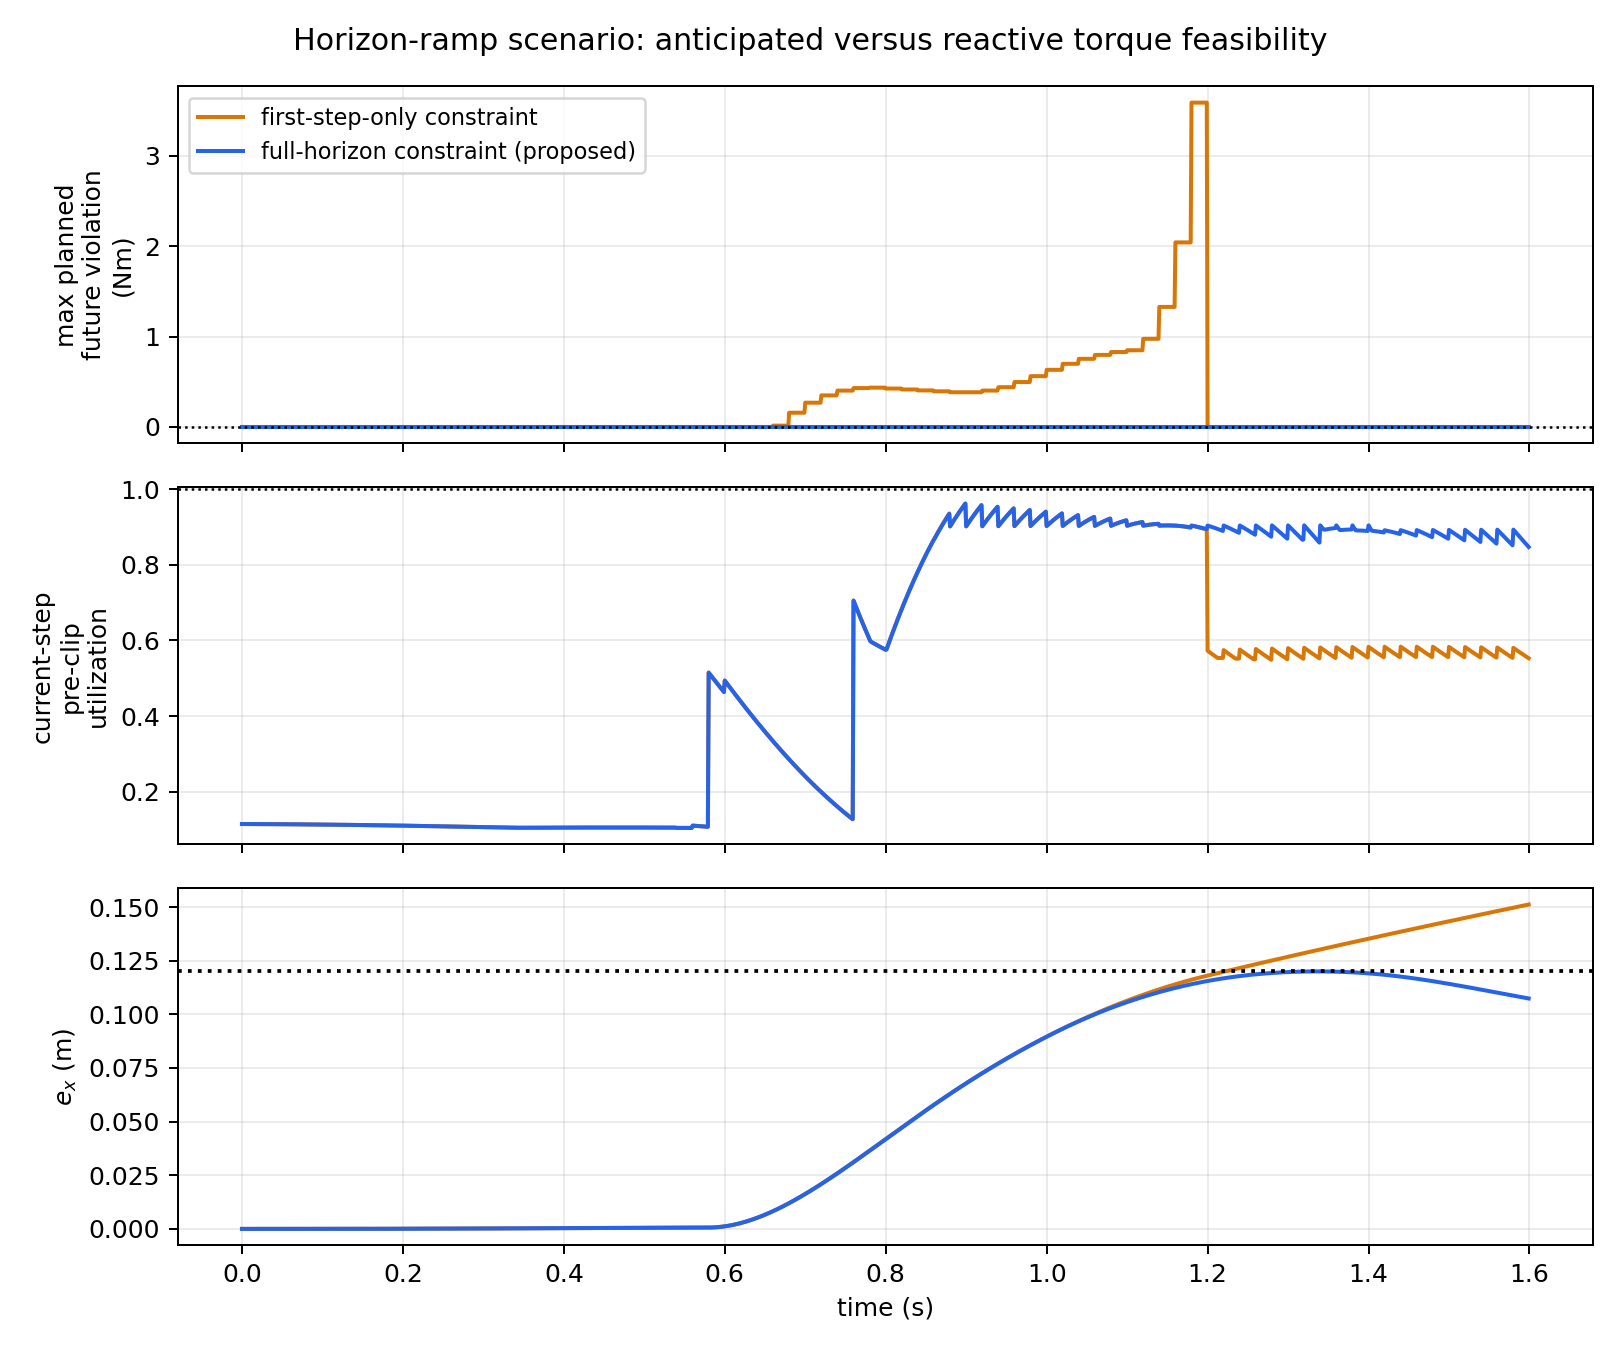
\includegraphics[width=\columnwidth]{horizon_ramp_results.png}
\caption{时域斜坡场景：仅约束第一步的方案眼见当下合法，却径直走向一个非法的未来；全时域约束方案则提前预见到了这一点。}
\label{fig:horizon}
\end{figure}

图~\ref{fig:horizon}隔离出了为何“预见”是一种与“反应式限制”不同的约束方式，而不只是对后者的一种改良：
\begin{itemize}
\item manager 的时域各行直接查询该场景中已排定的执行器预算下降计划，因此图~\ref{fig:horizon}展示的是在一个已知未来约束下、时域方案与单步方案之间的机制差异，而不是对一个未知约束的预测能力。
\item 仅约束第一步的方案，其预测中的未来力矩违反达到 3.587~Nm；全时域约束方案则始终保持为零。
\item 仅约束第一步方案的 QP 只有 75\% 的更新是可行的，而全时域约束方案则为 100\%。
\item 由此产生的 31.180~mm 工作空间超限，完全发生在那 25\% 不可行的情形中，是由第~\ref{sec:predictivecorrection}节的反应式后备方案介导产生的（在 QP 可行的情况下为 0.000~mm）。
\end{itemize}

\begin{figure}[t]
\centering
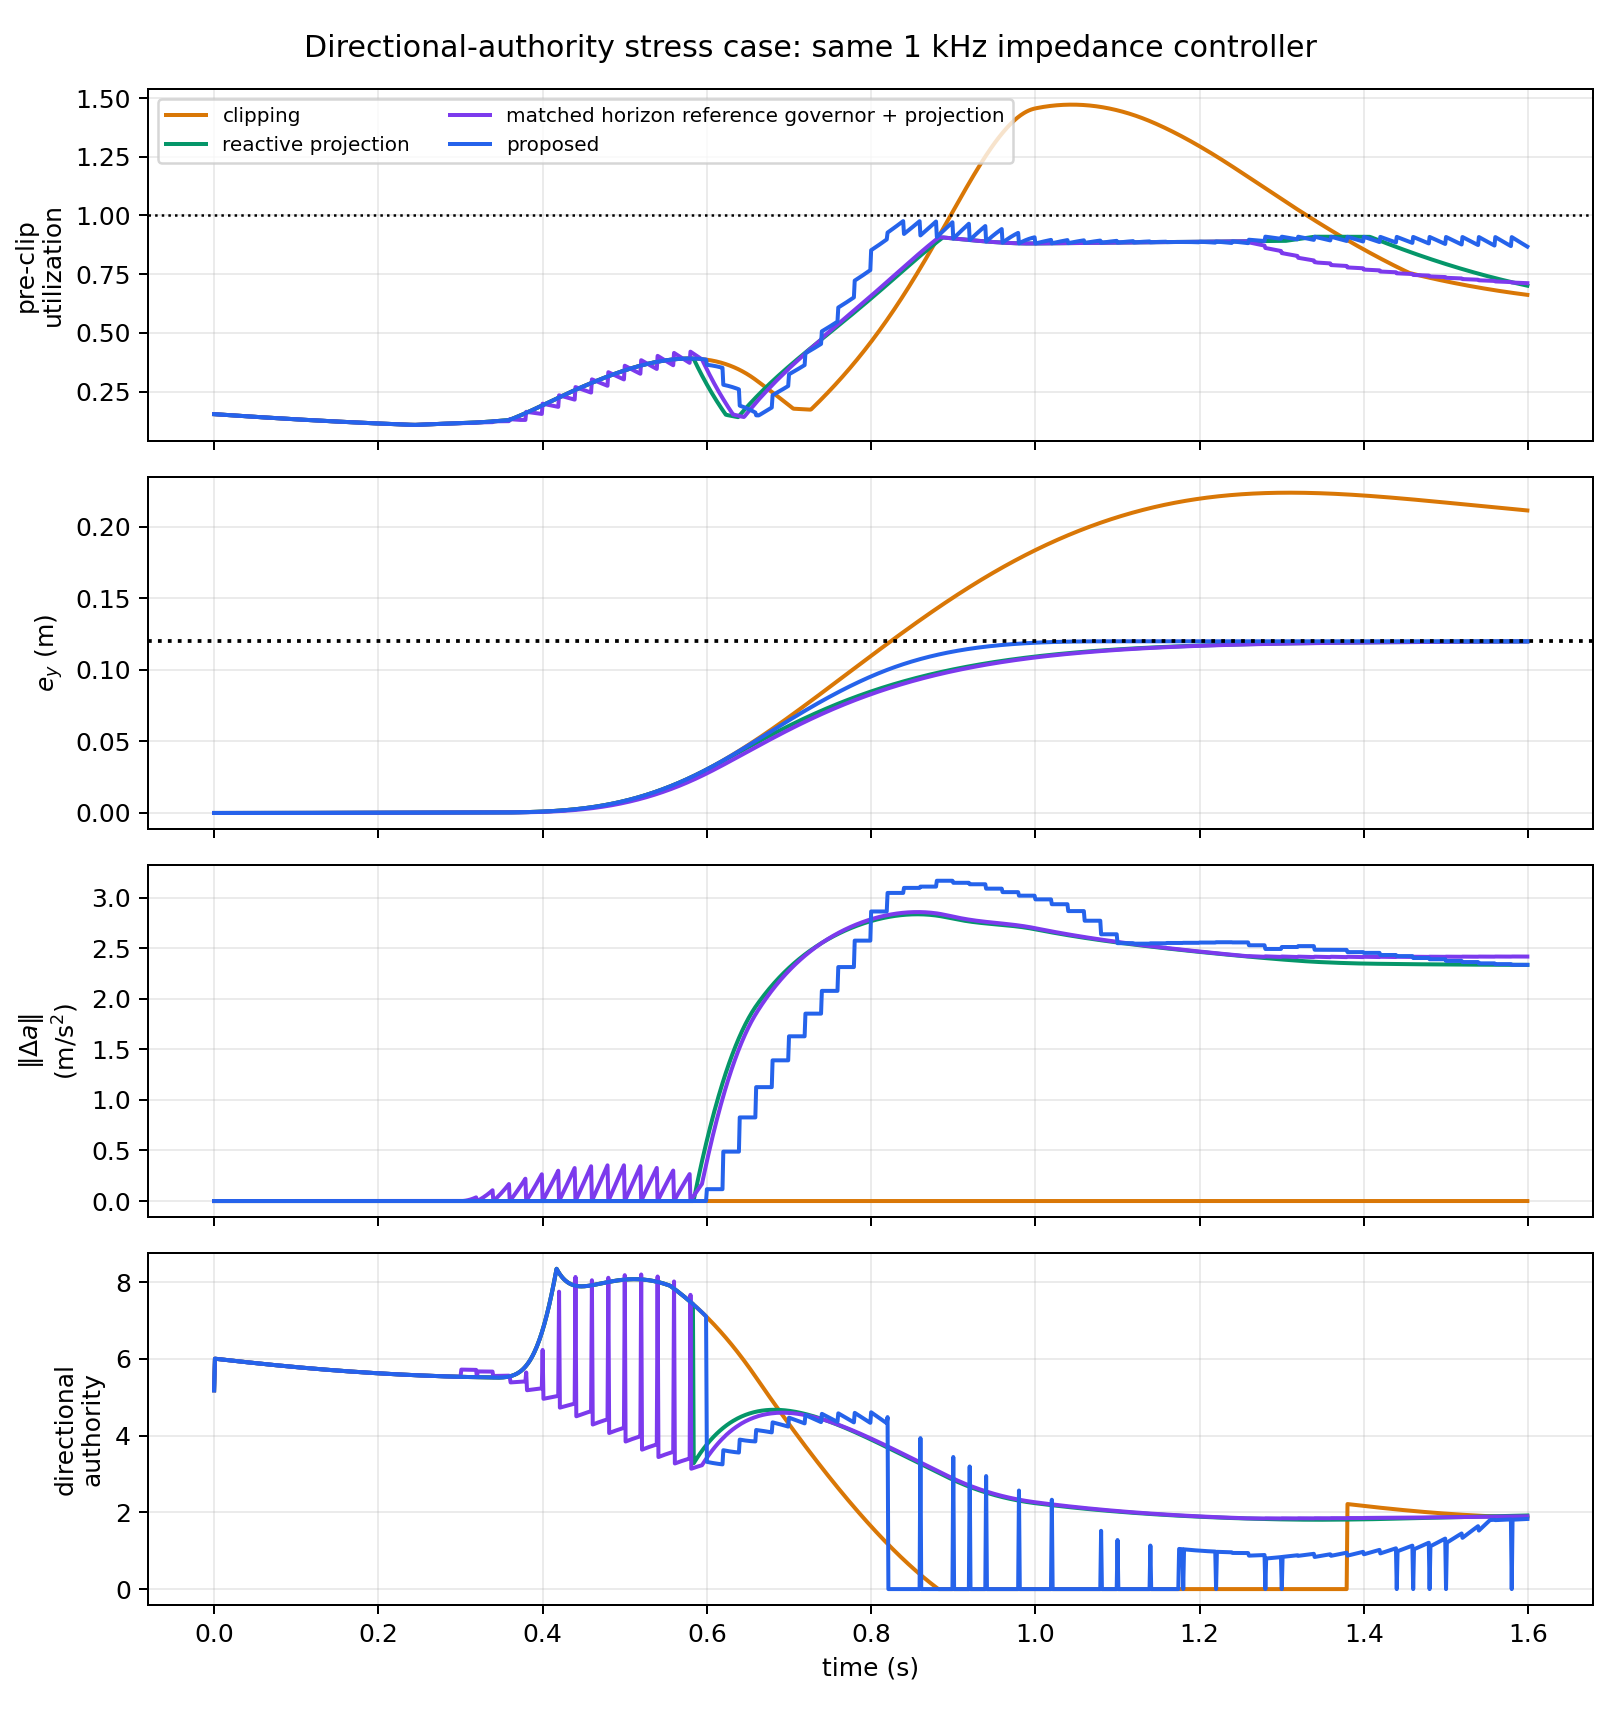
\includegraphics[width=0.8\columnwidth]{directional_authority_results.png}
\caption{在一个常见阻抗控制器接口下的方向性权限压力案例。}
\label{fig:directional}
\end{figure}

图~\ref{fig:directional}展示了方向性权限压力案例。直接截断同时超出了可行请求集与工作空间边界。预测式方法介入得更早，向量修正方案在保持工作空间约束的同时，留下了一个可见的介入残差。沿扰动方向测量（度量定义见附录~\ref{app:params}），本文所提出 manager 的权限在轨迹的约五分之一时段内降为零，而被施加的请求在全程始终满足工作空间约束；反应式投影与匹配的时域参考调节器，在整次运行中沿这一方向都保持正的权限（最小值分别为 1.82 和 1.87~m/s$^2$）。

\begin{figure}[t]
\centering
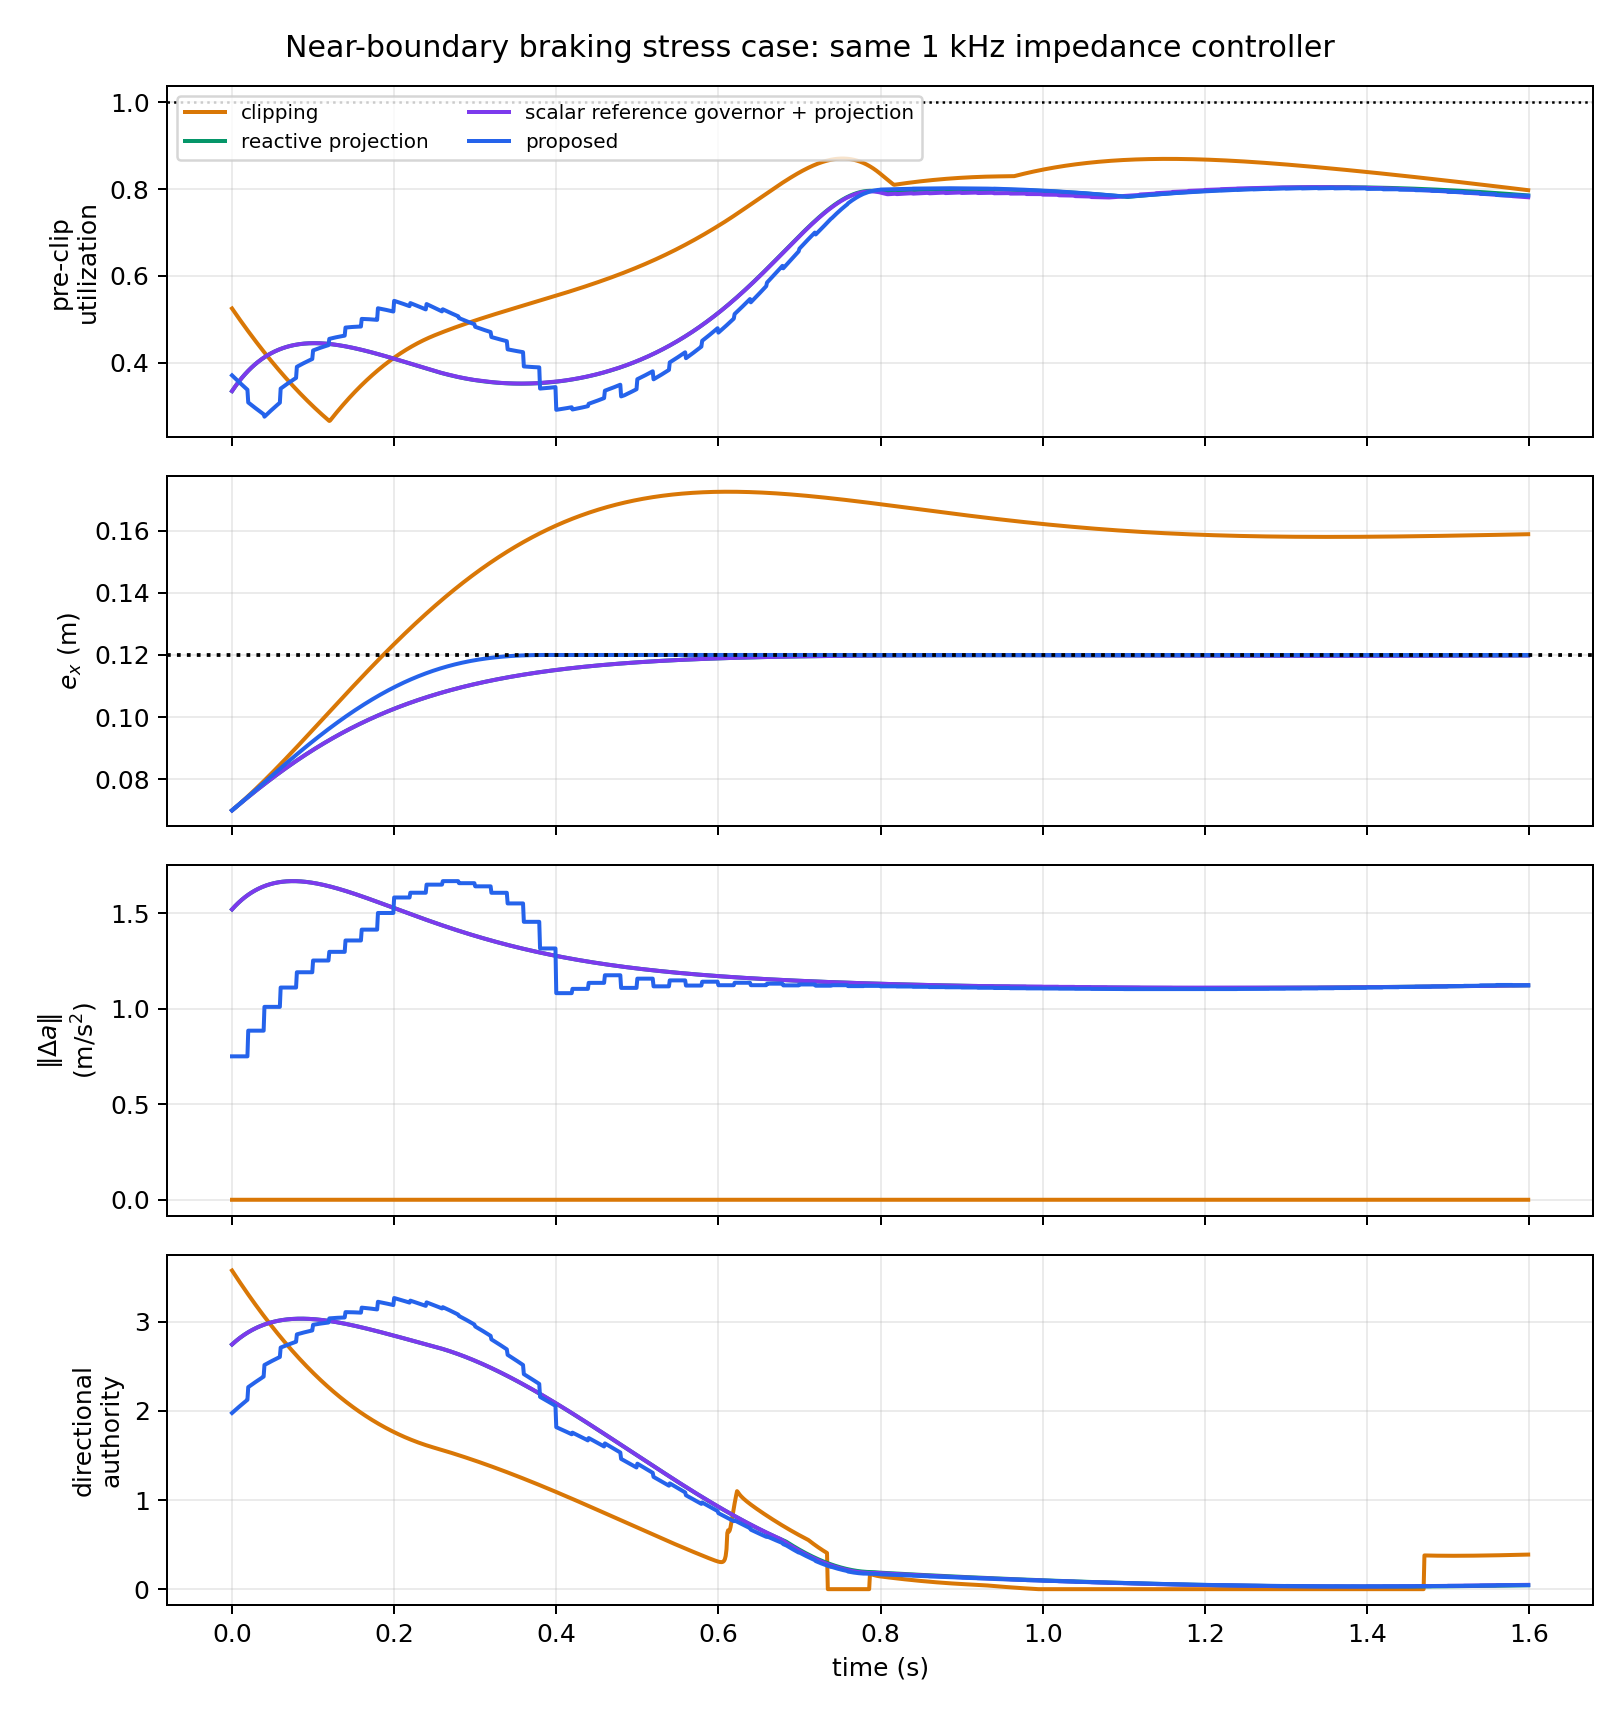
\includegraphics[width=0.8\columnwidth]{near_boundary_braking_results.png}
\caption{近边界制动压力案例；本文并未从该轨迹推断出任何可行核。}
\label{fig:braking}
\end{figure}

图~\ref{fig:braking}展示了近边界制动：在执行器预算不断收缩的情况下，一个朝外的速度接近位置边界。直接截断会越过边界并停在边界之外。反应式投影、匹配的时域轨迹参考调节器加投影，以及本文提出的 manager，三者都能把位置制动在边界处。由于本文并未计算可行核或终端不变集，这一结果仅支持“有限时域约束处理有效”这一结论。

表~\ref{tab:scenarios}报告了在其余七个场景下，截断、匹配的时域轨迹参考调节器，以及所提出的行为坐标 manager 三者的表现。该调节器使用与本文相同的实现模型、20~ms 更新周期、0.24~s 时域、执行器限制时间表、收紧机制，以及 1~kHz 的最终投影。它搜索的是一个标量参考乘子，而本文提出的 manager 则在每个时域步上优化一个加速度向量。这使它成为一个 ERG 风格、同模型的数值对比对象，而不是对 \cite{r17} 的 Lyapunov/动态安全裕度算法的精确复现。

在名义上成功的案例中，两种预测式架构给出了相同的定性结果：都消除了截断前的超限，并把工作空间超限控制在数值尺度以内。二者的介入提前量最多相差 33~ms，与两次共享的 20~ms manager 更新周期相当；时域长度为 $N\Delta t=0.24$~s。修正 RMSE（调节器/所提方法）在缓慢饱和、方向性崩溃与近边界制动三个场景下，分别为 $1.124/1.060$、$1.389/1.401$ 与 $0.878/0.844~\mathrm{m/s^2}$；在时域斜坡隔离案例中为 $0.695/0.506~\mathrm{m/s^2}$。由此可见，在这四个案例中的三个上，向量接口对被请求行为的改动更小，而标量调节器仅在方向性崩溃场景中略优。这是一种与表示方式相关的权衡证据，而不是相对于 \cite{r17}、广义动作调节器 \cite{r18} 或预测安全滤波器 \cite{r5,r16} 的普遍优越性证据。

\begin{table*}[t]
\caption{同模型场景对比。C/G/P 分别表示截断/匹配时域轨迹参考调节器/所提出的行为坐标 manager}
\label{tab:scenarios}
\centering
\footnotesize
\setlength{\tabcolsep}{4pt}
\begin{tabular}{@{}lccccc@{}}
\toprule
场景 & \shortstack{截断前\\C/G/P (Nm)} & \shortstack{工作空间\\C/G/P (mm)} & \shortstack{提前量\\G/P (s)} & \shortstack{P\\可行率} & \shortstack{P\\审计} \\
\midrule
无饱和 & 0.000 / 0.000 / 0.000 & 0.000 / 0.000 / 0.000 & -- / -- & 100\% & 通过 \\
缓慢饱和 & 0.000 / 0.000 / 0.000 & 78.970 / 0.000 / 0.001 & 0.399 / 0.414 & 100\% & 通过 \\
突发扰动 & 7.151 / 10.236 / 11.879 & 0.000 / 0.000 / 0.000 & 0.086 / 0.084 & 92.5\% & 未通过 \\
方向性崩溃 & 0.708 / 0.000 / 0.000 & 103.868 / 0.000 / 0.003 & 0.307 / 0.340 & 100\% & 通过 \\
近边界制动 & 0.000 / 0.000 / 0.000 & 52.537 / 0.000 / 0.011 & 0.574 / 0.568 & 100\% & 通过 \\
模型失配 & 12.453 / 1.190 / 2.018 & 190.904 / 160.711 / 197.006 & 0.542 / 0.633 & 45.0\% & 未通过 \\
预见失配 & 19.777 / 3.537 / 4.428 & 190.513 / 357.209 / 346.871 & 0.173 / 0.169 & 40.0\% & 未通过 \\
\bottomrule
\end{tabular}
\\[2pt]
\raggedright\footnotesize 表 II. 同模型场景对比。C/G/P 分别表示截断/匹配时域轨迹参考调节器/所提出的行为坐标 manager。提前量是相对于每种预测式方法自身第一次名义限制事件而言的；附录~\ref{app:params}说明了这一共享事件诊断指标。
\end{table*}

\textbf{负面案例。} 在四个成功的压力案例中，QP 可行率均为 100\%，但在突发扰动、模型失配与预见失配下，分别只有 92.5\%、45.0\% 与 40.0\%，其余超限大部分由第~\ref{sec:predictivecorrection}节的反应式后备方案承担。在预见失配下，修正量所依据的力预报，在时域内漏掉了一次符号反转，工作空间超限从 190.513 升到 346.871~mm——比什么都不做还要差；模型失配的情况类似，从 190.904 恶化到 197.006~mm，因为可行几何是沿着一个错误的滚动预测组装出来的。在突发扰动下，本文所实现的预见方式把测得的力保持不变，因此一次未经宣告的冲击，会把截断前超限从 7.151 推高到 11.879~Nm，尽管最终投影仍然保证了施加力矩的合法性。审计机制拒绝了这三个案例，精确标出了定理~\ref{thm:transfer}的前提在何处未被满足。

\subsection{控制器接口替换}

\begin{figure}[t]
\centering
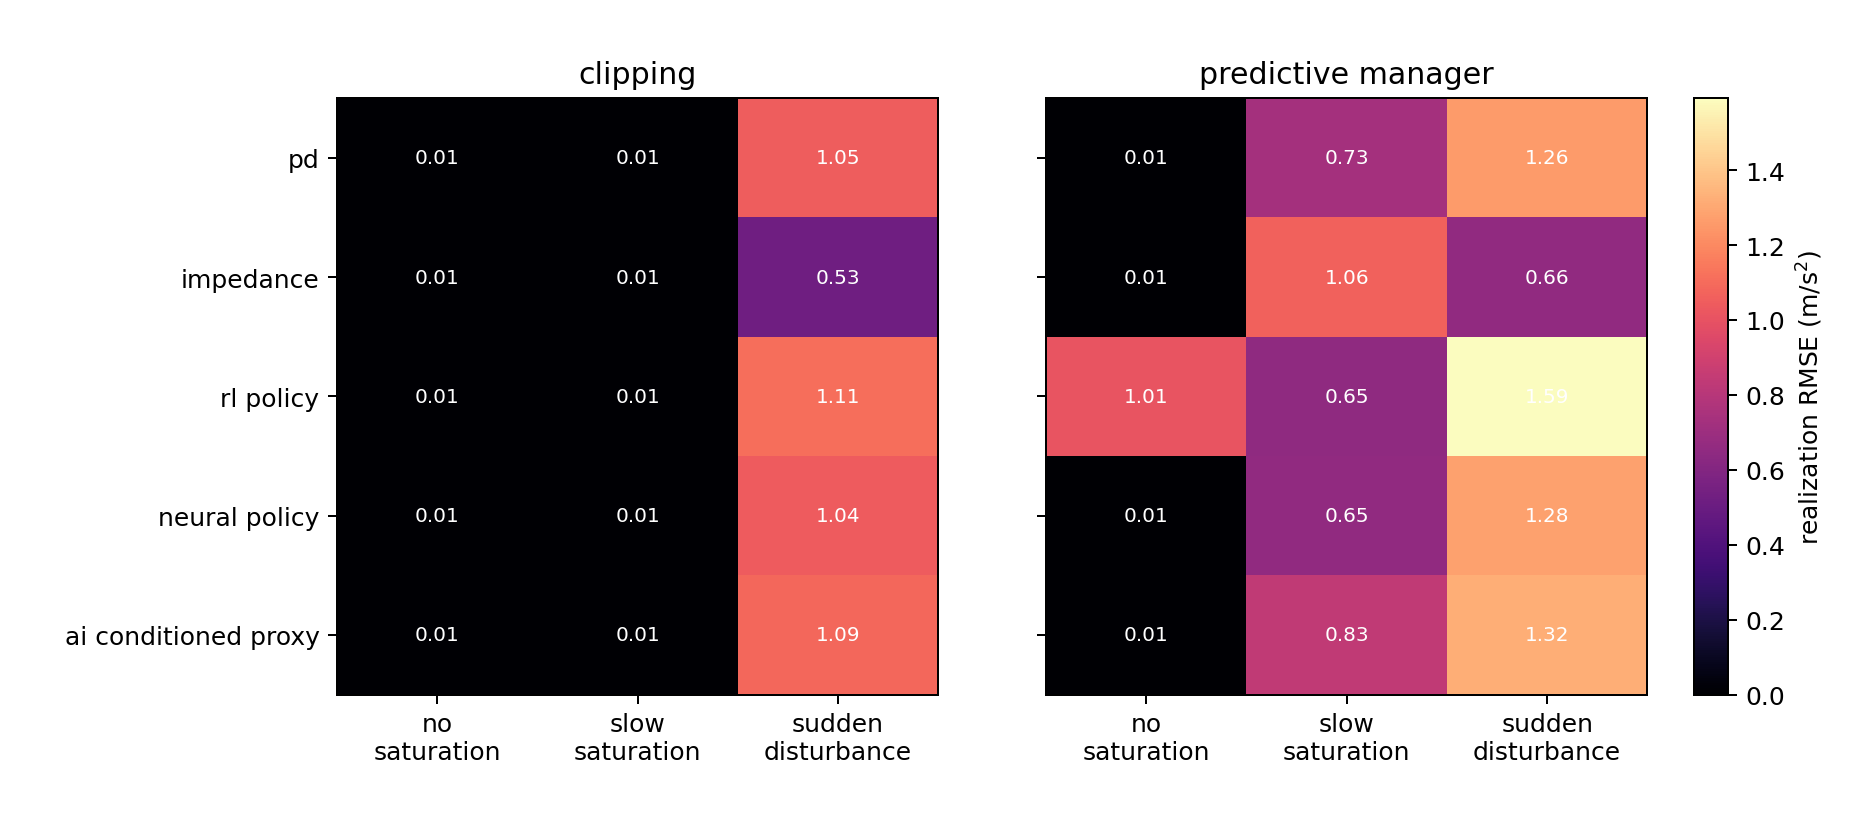
\includegraphics[width=\columnwidth]{controller_transfer.png}
\caption{五种名义控制器接口下的行为实现残差。}
\label{fig:controllers}
\end{figure}

如图~\ref{fig:controllers}所示，manager 的构造与权重在各接口之间保持不变。在无饱和条件下，五个控制器中有四个的修正 RMSE 低于 0.01~m/s$^2$；小型进化策略策略是例外，约为 $1.01~\mathrm{m/s^2}$（偏置来源见附录~\ref{app:params}）。manager 把状态保持在工作空间盒约束内，但此时它做的是补偿一个有偏置的接口，而不是保持未激活状态。该案例被保留下来，作为一个接口压力测试——本架构并不打算修复行为策略本身的质量，尽管其运行约束可能会顺带拒绝一个有偏置的请求。

表~\ref{tab:controllers}把 manager 的刻意修正量（$a_{\mathrm{req}}-a^0$）与跟踪缺陷 RMSE（$a_{\mathrm{actual}}-a_{\mathrm{req}}$）区分开来，后者与认证迁移的关系最为直接。跟踪缺陷在每种接口下都是 $0.0111~\mathrm{m/s^2}$——这是一个固定的、与控制器无关的未建模误差下限，因为在缓慢饱和下没有截断被激活——而修正 RMSE 则随每个控制器的实际请求而变化。全部五个案例都通过了审计。

\begin{table}[t]
\caption{缓慢饱和下的控制器替换}
\label{tab:controllers}
\centering
\footnotesize
\setlength{\tabcolsep}{3pt}
\begin{tabular}{@{}lcccc@{}}
\toprule
接口 & \shortstack{修正\\RMSE (m/s$^2$)} & \shortstack{跟踪缺陷\\RMSE (m/s$^2$)} & \shortstack{工作空间\\超限 (mm)} & 审计 \\
\midrule
PD & 0.726 & 0.0111 & 0.001 & 通过 \\
阻抗 & 1.060 & 0.0111 & 0.001 & 通过 \\
训练策略 & 0.652 & 0.0111 & 0.016 & 通过 \\
拟合神经网络策略 & 0.649 & 0.0111 & 0.001 & 通过 \\
条件化运动基元 & 0.830 & 0.0111 & 0.006 & 通过 \\
\bottomrule
\end{tabular}
\end{table}

\subsection{跨实现映射的采样式接口审计}
\label{sec:sampled}

\begin{table}[t]
\caption{与定理~\ref{thm:transfer}三个条件相关联的采样式起止点量}
\label{tab:audit}
\centering
\footnotesize
\setlength{\tabcolsep}{3pt}
\begin{tabular}{@{}lccc@{}}
\toprule
实现映射 & \shortstack{最大 T3 缺陷\\$\ell_\infty$ (m/s)} & \shortstack{最小 T1\\松弛量 (Nm)} & \shortstack{最小 T2\\松弛量 (Nm)} \\
\midrule
平面 2R & 0.006815 & 0.007604 & 0.143756 \\
FR3 启发替代模型 & 0.006796 & 0.003888 & 0.646664 \\
六轴机械臂替代模型 & 0.006796 & 0.004871 & 0.707748 \\
\bottomrule
\end{tabular}
\end{table}

每条记录按一次可行的 manager 更新索引，排除紧随一次不可行（后备）求解之后的节拍，因为定理~\ref{thm:transfer}针对的是经 QP 优化过的方案。(T1) 与 (T2) 在区间开始处求值，使用 manager 自身对时域第一步的预测 $\hat\tau_0$，以及由同一个请求所实现的力矩。二者使用相同的状态、力与请求，但数值上并不相等，因为二者之间的差距正是 (T1) 所约束的对象。(T2) 一栏是该节拍第一步的松弛量，而不是本文其他地方所报告的时域内最小值。(T3) 使用的是在\emph{下一次} manager 更新时观测到的物理状态。因此该表报告的是一次采样式的起止点审计——来自无饱和与缓慢饱和两种跨实现运行的、每个机器人 316 条记录——而不是主张其区间起点处的 (T1) 与 (T2) 值，在中间那 20~ms 内、快速控制器与实现映射不断演化的过程中持续成立。

表~\ref{tab:scenarios}与表~\ref{tab:controllers}中的通过/未通过标签，来自一个独立的、更宽泛的、覆盖每一个 1~kHz 快循环采样点的非配对审计。它使用一个欧几里得（T3）界，相对表~\ref{tab:audit}的 $\ell_\infty$ 值更为保守，核查力矩误差包络，并直接要求已实现的截断前力矩落在未收紧的执行器盒约束之内。因此，“每条通过案例的轨迹全程截断前力矩都合法”这一说法，是由快循环层面的检查所支撑的，而不是仅从表~\ref{tab:audit}的 manager 更新快照中推断出来的。表~\ref{tab:audit}显示，三种实现映射下的采样松弛量均为正：(T3) 缺陷始终低于 0.03~m/s 的认证裕度，而 (T1) 与 (T2) 相对于 $\bar\delta_\tau(a,F_h)$（附录~\ref{app:params}）仍留有余地。真实被控对象的系数对 manager 是留出的，也不是通过缩放该界自身的波形生成的。尽管如此，系数盒与留出的被控对象本身都仍然是合成的；这比一个自我包络的一致性检验更有力，但仍弱于一个独立辨识出的物理不确定性集合。

\subsection{消融汇总与计算量}
\label{sec:ablation}

\begin{figure}[t]
\centering
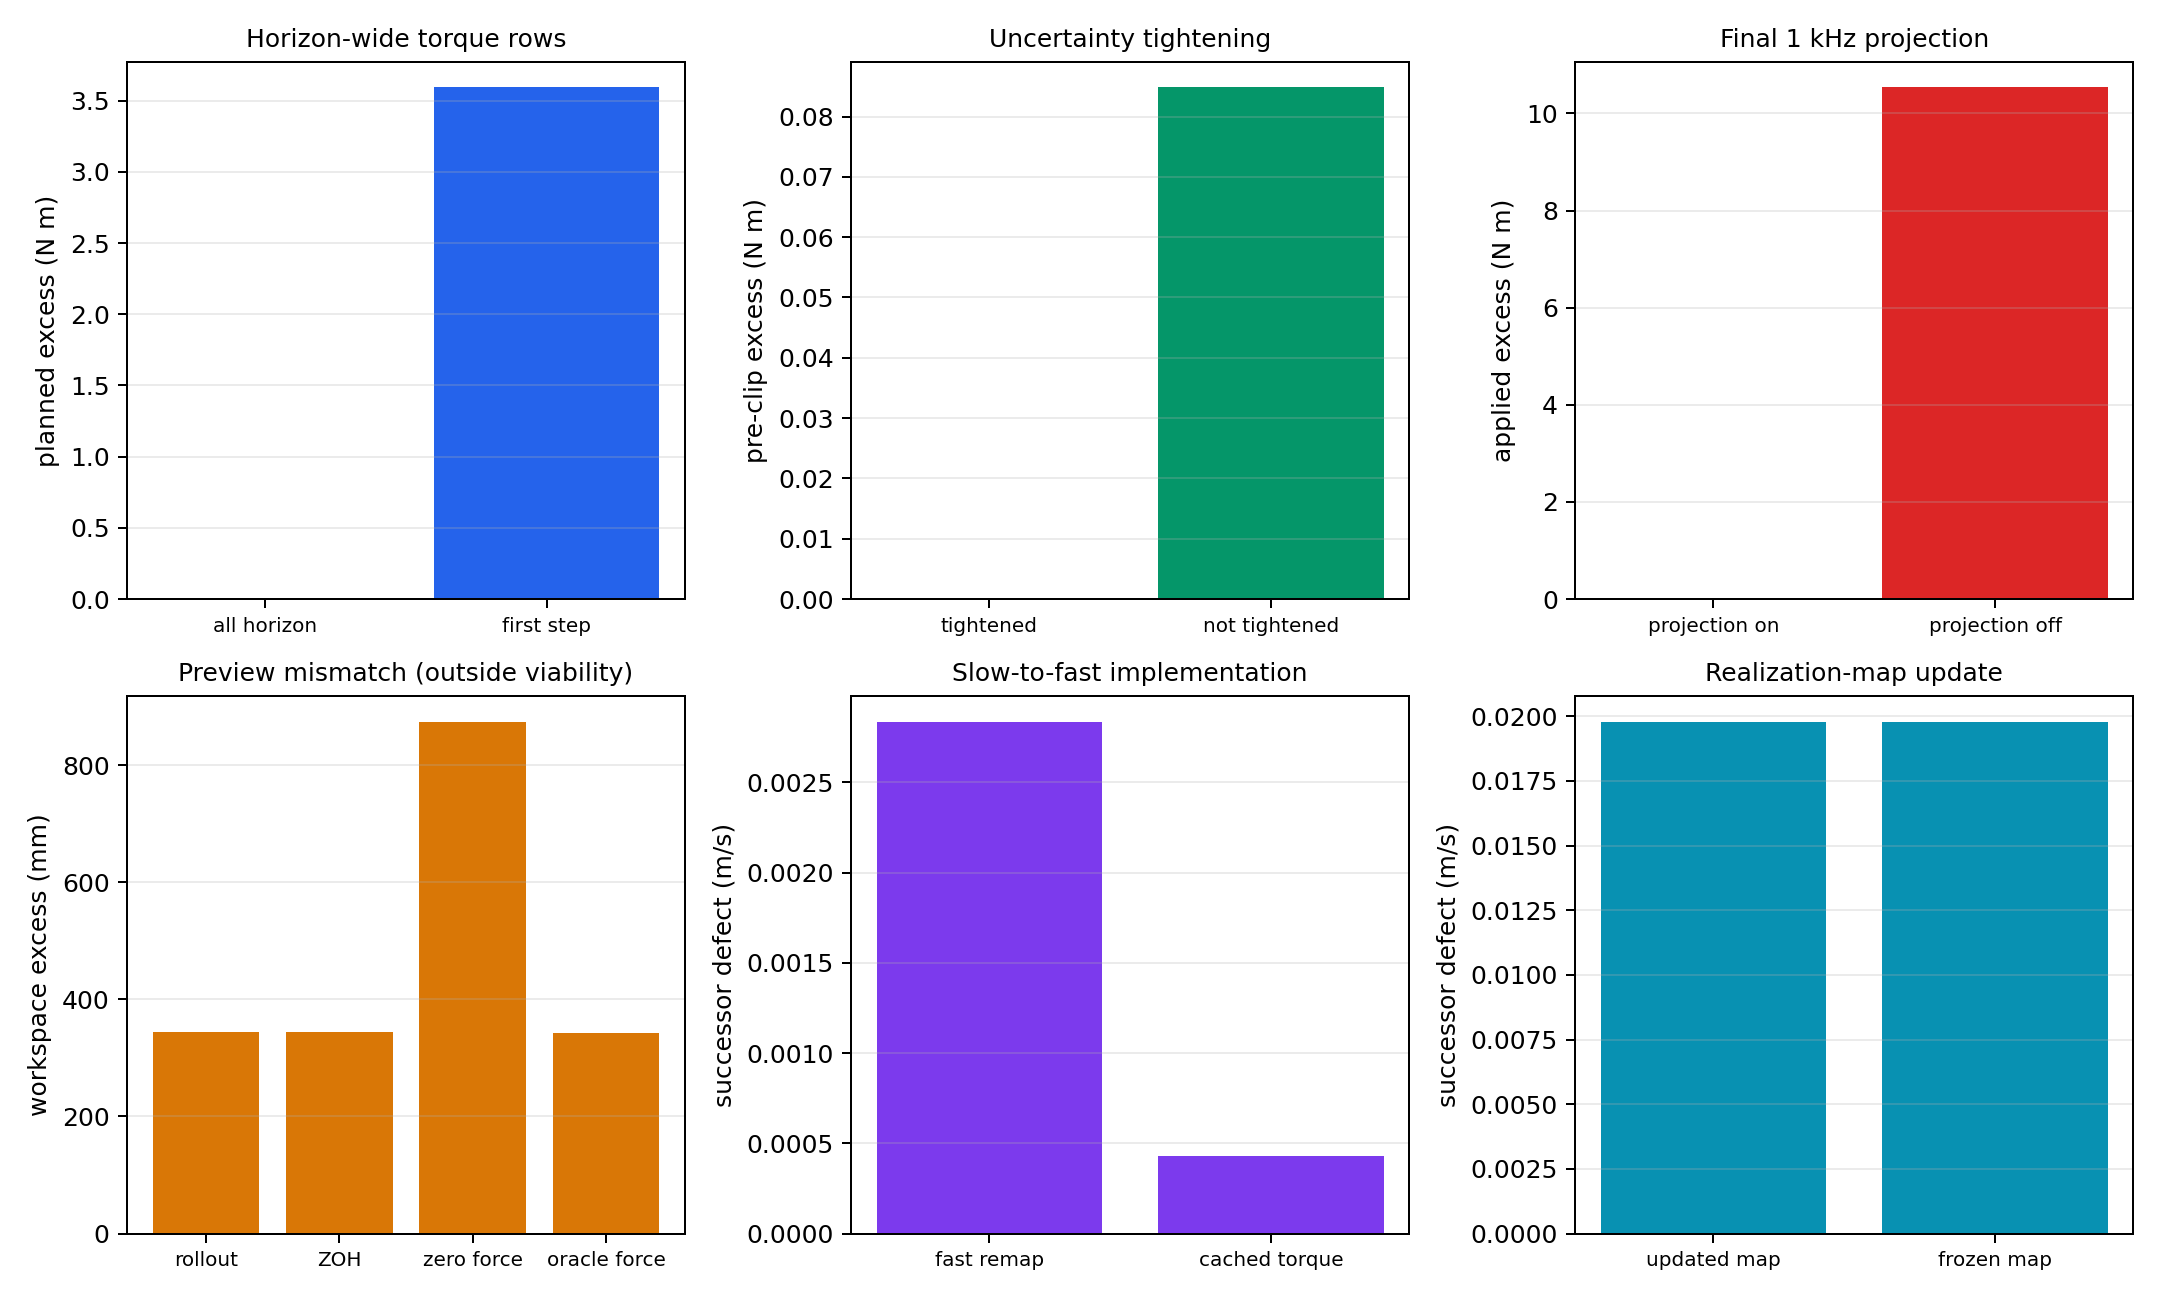
\includegraphics[width=\columnwidth]{ablation_summary.png}
\caption{对预测式与快速通道实现选择所做的成对消融实验。}
\label{fig:ablation}
\end{figure}

图~\ref{fig:ablation}隔离出了本文的四项核心设计选择。全时域强制约束使时域斜坡场景下的 QP 保持可行，并消除了仅约束第一步所遗留的 3.587~Nm 计划违反。去掉不确定性收紧会产生 0.0958~Nm 的截断前超限；去掉最终投影，会在突发扰动下产生 10.456~Nm 的施加后超限。在专门的速度约束案例中，强制执行 $\mathcal K_v$ 把峰值速度限制在 0.5678~m/s，而不强制执行时为 0.5968~m/s。附录~\ref{app:params}给出了完整的 17 项消融清单、次要结果，以及墙钟计算耗时数据。

\section{讨论}

这些实验支持的是一个接口层面的主张，而不是“这个新的安全控制器对任何机器人都有效”这一主张。行为坐标优化与经验审计阈值，在所实现的各控制器接口与各实现映射之间保持不变，而每个映射各自重建自己的可行集与误差界。这一分离正是本文所展示的贡献。它并不能确立“一个动作调节器或预测安全滤波器不能使用同样的坐标”这一结论；表 I 明确指出了这一尚未解决的关系。

参考调节器、动作调节器与预测安全滤波器，同样可以采用相同的行为坐标。本实现所贡献的，是一条显式的软件与验证边界：一侧是行为请求与已认证动作集；另一侧是机器人专属的力矩映射、不确定性裕度与后继审计。在本研究中，速度认证 $(\mathcal S_v,\mathcal K_v,\epsilon_v)$ 被刻意设计得很简约。它所要求的物理约束——真实的单步失配始终落在 $\epsilon_v$ 之内——是沿实验轨迹采样得到的，而不是在整个工作空间上被独立辨识出来的。力矩审计把已声明的系数盒与确定性留出的真实被控对象系数区分开来，但二者仍然都是合成的。因此，本文的结果验证的是“在一个预先给定的不确定性类别内，对一个留出扰动的处理效果”，并展示了“在人为构造的失配下审计机制会拒绝该案例”；它们并未辨识出一个在整个工作空间上成立的物理不确定性集合。

最终的高速率投影是必不可少的，但不应与行为保留混为一谈：截断保护的是执行器，却使被请求行为的精确实现失效。定理~\ref{thm:transfer}记录的是“截断保持未激活、且速度结论对一次迁移成立”的充分条件。失配实验表明这些性质会出现分歧。匹配时域参考调节器的对比表明，二者具有相当的约束处理能力，以及一种与场景相关的修正权衡。由于本文既未包含终端不变集，也未包含对 \cite{r17}、一个广义动作调节器，或一个预测安全滤波器的精确实现，这些结果不应被解读为递归安全性证据，也不应被解读为广泛意义上的比较优越性证据。

三种实现映射测试的是在同一降阶模型类别内的软件替换与不同的执行器几何形状。它们并不能证明一个已辨识的不确定性契约或认证，能够在真实物理机器人动力学之间迁移。推论~\ref{cor:tworate}与第~\ref{sec:predictivecorrection}节的时域漂移项，指出了这样一个主张所额外需要的界；本文的仿真都没有辨识出这两个界。

\section{结论}

本文提出了一种面向预测式饱和管理的行为坐标实现接口。名义控制器以其较高的伺服节拍暴露出一个任务加速度请求；一个较慢的 manager 预测机器人专属的可实现性丧失，并在截断真正被需要之前修改该请求。预测式监督本身已是既有的现有工作。本文的贡献在于给出了一种具体的分离方式：一侧是可复用的、行为一侧的请求与动作集；另一侧是必须被重建并审计的、机器人专属的对象——加速度到力矩的映射、执行器裕度、不确定性界与工作区域。一个最小化的、经速度认证的动作集，作为一种存在性见证被强制在 QP 内部执行，而定理~\ref{thm:transfer}则给出了相应的单步实现契约。

在 111 次确定性降阶仿真运行中，全时域强制约束消除了仅约束第一步这一变体所遗留的一个计划中的未来违反，同一接口接受了五种名义控制器形式。一次采样式审计，在为三种机器人替代模型保留各自不同实现映射的同时，应用了同一个行为失配阈值。缓慢饱和、方向性权限崩溃与近边界制动，在被测试的区域内都得到了妥善处理。一个匹配的 ERG 风格轨迹参考调节器，以相当的效果处理了这些约束；向量式行为修正方案，在四个成功案例或时域隔离案例中的三个上具有更低的修正 RMSE，但在方向性崩溃案例中并非如此。突发扰动与严重失配则会使该契约失效，并常常使 QP 变得不可行，此时只剩下反应式后备方案与最终投影可用。这些结果确立的是：本接口能够正常运行、暴露出一个可测量的表示方式权衡，并按设计拒绝不满足前提的情形；它们并未确立相对于调节器或安全滤波器架构的普遍优势。

下一步具有决定性意义的评测，是对饱和感知 ERG、广义动作调节器，或预测安全滤波器实现的精确复现，以及在完整刚体或真实硬件实现上、使用独立辨识出的误差界所进行的验证。向位置认证与递归可行性方向的扩展，则是另外的理论方向。

\appendices
\section{基准测试参数}
\label{app:params}

本附录列出了复现第~\ref{sec:experiments}节数字所需的常数，包括完整的消融清单；完整的实现映射函数 $H(x)$、$\tau_{\mathrm{base}}(x)$、学习策略的权重，以及各场景的时间表，都在随本文一并发布的仿真代码中。

\textbf{共享常数}（\texttt{BenchmarkConfig}，\texttt{simulation/saturation\_benchmark.py}）：快循环周期 $T_f=1$~ms，manager 周期 $\Delta t=20$~ms，时域长度 $N=12$，单次试验时长 1.6~s，工作空间盒约束 $\mathrm{pos}_{\max}=0.12$~m，速度盒约束 $v_{\max}=0.60$~m/s，加速度界 $a_{\max}=12.0~\mathrm{m/s^2}$，加速度变化率界 $\dot a_{\max}=120.0~\mathrm{m/s^2/s}$，认证/审计裕度 $\epsilon_v=\epsilon_{\mathrm{audit}}=0.03$~m/s，代价权重 $W=1.0\cdot I$、$W_\Delta=0.025\cdot I$，OSQP 容差 $10^{-5}$。由此得到 $\epsilon_v/\Delta t=1.5~\mathrm{m/s^2}$，远低于 $a_{\max}$——这正是第~\ref{sec:certificate}节中 $\mathcal K_v$ 非空性所依赖的具体裕度。

\textbf{实现映射}（力矩限制单位为 Nm，质量单位为 kg）：所列出的每一个力矩限制数组，都是一个对称盒约束的正幅值 $L$，即 $\tau_{\min}=-L$、$\tau_{\max}=L$。平面 2R——2 个关节，$L=[9.0,7.5]$，质量 2.2；FR3 启发替代模型——7 个关节，$L=[16.0,13.0,12.0,15.0,6.0,6.0,4.5]$，质量 3.0；六轴机械臂替代模型——6 个关节，$L=[12.0,10.0,9.0,8.5,5.5,4.5]$，质量 2.6。交互误差界 $\bar\delta_\tau$ 使用每关节 0.03~Nm 的基础项，以及下文与 $H$ 相关的项，其中 $H_0=H(x)$ 是在每个映射各自的零状态构型处求值一次得到的。

\textbf{跨实现审计细节。} 在仿真的真实被控对象被实例化之前，manager 的逐关节界被固定为
\begin{align*}
\bar\delta_\tau^{(j)}
=\ &s_{\mathrm{mm}}\Bigg(\underbrace{0.03}_{\text{Nm，基础项}} \\
&+0.008\sum_{k}\max\!\left(\left|H_0\right|_{jk},0.25\right)\left|a_k-\frac{F_{h,k}}{m}\right|\Bigg),
\end{align*}
其中 $s_{\mathrm{mm}}$ 是该场景的失配尺度乘子（本文所报告的跨实现案例中为 1.0，在第~\ref{sec:experiments}节其他地方的模型失配案例中最高可达 2.4），在整个审计中取值范围为 0.0300 到 0.0926~Nm；这是第~\ref{sec:realizable}节中与动作相关的界 $\bar\delta_\tau(a,F_h)$，而不是 QP 自身更保守的 $\bar\delta_\tau^{\mathrm{QP}}$。随后，留出的真实被控对象分别使用种子 31、37 与 41，为平面 2R、FR3 启发以及六轴机械臂三种映射生成。它们各自独立的系数满足 $|c_H|\le0.0065<0.008$，基础误差幅值落在 $[0.012,0.027]$~Nm${}<0.03$~Nm 之内，相位与频率也是独立采样的；这些被实现出来的真实值从未被传递给 manager。表~\ref{tab:audit}直接报告了由此得到的 (T1) 与 (T2) 松弛量。这是在一个预先给定的合成系数盒内进行的确定性留出测试，而不是从物理数据中辨识出该系数盒。

\textbf{基线架构。} 反应式 1~kHz 投影：对当前步被收紧的力矩半空间，与一个相对度为二、衰减率 $\lambda=8$ 的盒式控制屏障函数半空间集合（\texttt{reactive\_state\_halfspaces}）的交集，做精确的欧几里得投影，即位置相关行为 $\mp a\le\pm2\lambda v+\lambda^2(\mathrm{pos}_{\max}\mp p)$，速度相关行为 $\mp a\le\lambda(v_{\max}\mp v)$。匹配时域轨迹参考调节器：在每个 manager 节拍，\texttt{governor\_scale} 使用二分法寻找最大的 $\alpha\in[0,1]$。对每个候选值，把状态沿全部 $N=12$ 步向前滚动，针对 $p+\alpha(p_r-p)$ 求值名义控制器，并核查与所提出 manager 相同的：已排定执行器限制、经不确定性收紧的力矩半空间、工作空间与速度界、测得力保持不变、模型、20~ms 更新周期，以及 0.24~s 时域。第一个被调节过的参考值会一直保持到下一个 manager 节拍，其请求的加速度经过与本文相同的反应式投影。这是一个受 \cite{r17} 启发、ERG 风格的同模型对比对象，但它直接搜索有限时域约束可行性，而不是复现 \cite{r17} 的 Lyapunov/动态安全裕度控制律。

\textbf{方向性权限度量。} $\alpha^+$（第~\ref{sec:reports}节）是所选方向 $y$ 的一个函数。图~\ref{fig:directional}报告的是沿固定的、外生扰动方向的取值，而不是 manager 自身的修正方向——后者是内生的，会随 manager 自身输出的变化而不连续地改变，因此在不同方法或不同时刻之间不能直接比较；二者都使用相同的半空间-射线构造方式。

\textbf{调节器搜索验证。} 匹配调节器对 $\alpha$ 使用二分法搜索，这假设可行性关于 $\alpha$ 是单调的。在本基准测试中该调节器被调用的全部 160 个 manager 节拍上，一个 201 点的密集网格检验没有发现任何非单调的情形。一项回归测试还进一步确认，其时域能够在一次已排定的限制下降到来之前提前削弱参考量，而一个单步版本此时还无法预见到这一点。

\textbf{控制器接口。} PD 与阻抗是解析形式的控制律。训练策略是一个用 $\tanh$ 压缩输出的小型单隐层网络，通过一个确定性进化策略拟合得到。拟合神经网络策略是一个具有 18 个单元的 $\tanh$ 隐层加线性输出头，通过最小二乘拟合阻抗律的示范数据得到（见 \texttt{saturation\_benchmark.py} 中的 \texttt{RLPolicyController}/神经控制器拟合）。条件化运动基元是一个跟踪基元条件化参考的 PD 伺服。

\textbf{训练策略的偏置（第~\ref{sec:experiments}节）。} 该进化策略策略有限的训练集，并没有对称地覆盖测试轨迹，因此保留了一个 $y$ 正方向的指令偏置；这是一个被观测到的泛化误差，而不是进化策略算法本身的特定缺陷。

\textbf{计算量。} 在被保存的运行记录中，manager 与快速通道所观测到的最坏墙钟耗时最大值，均低于各自的名义周期（分别为 20~ms 与 1~ms），中位数求解时间也都明显低于各自预算。这些都是在一台开发机器上测得的墙钟计算耗时，而不是一个实时性保证；由于它们在不同运行之间是非确定性的，公开的 \texttt{results/all\_experiment\_metrics.json} 才是权威记录，而不是本文引用的任何具体数字。仿真器本身每一步都精确地把物理状态向前推进 1~ms，并不对“错过截止时限时调度器丢弃或延迟某一步”这种情况建模。一个具备显式调度策略的硬实时实现，是未来的工作。

\textbf{案例统计。} 这 111 个案例，由 40 个场景案例、30 个控制器接口案例、24 个跨实现案例，以及归为八个族的 17 项消融组成。这 40 个场景案例，是八个场景各自在五条通道下评测得到的：四种架构——直接截断、一个反应式 1~kHz 投影、匹配时域轨迹参考调节器加同一个反应式投影，以及所提出的、带最终投影的全时域行为坐标修正——外加一条不带力矩投影的无约束名义参考通道。压力场景包括：无饱和、缓慢饱和、突发扰动、方向性权限崩溃、近边界制动、模型失配、预见失配，以及一个直接以图~\ref{fig:horizon}形式报告、并用于第~\ref{sec:ablation}节约束宽度消融的时域斜坡场景。第九个场景，从 $\mathcal S_v$ 内部、靠近其收紧边界处开始，仅用于速度认证消融实验，不进入场景矩阵或跨实现矩阵。

\textbf{完整消融清单。} 全部消融实验均使用 FR3 启发替代模型与阻抗控制器。

\begin{table}[t]
\caption{完整消融清单}
\label{tab:ablations}
\centering
\footnotesize
\setlength{\tabcolsep}{3pt}
\begin{tabular}{@{}rp{1.5cm}p{1.7cm}p{2.9cm}@{}}
\toprule
\# & 场景 & 变体 & 改变的元素 \\
\midrule
1 & 时域斜坡 & 完整 & 完整的所提出 manager \\
2 & 时域斜坡 & 仅第一步力矩 & 力矩约束仅作用于时域第一步 \\
3 & 缓慢饱和 & 缓存完整力矩 & 在两次 manager 更新之间保持完整力矩指令不变 \\
4 & 突发扰动 & 完整 & 完整的所提出 manager \\
5 & 突发扰动 & 无最终投影 & 关闭 1~kHz 力矩投影 \\
6 & 模型失配 & 完整 & 完整的所提出 manager \\
7 & 方向性崩溃 & 完整 & 完整的所提出 manager \\
8 & 方向性崩溃 & 无收紧 & 在预测式约束中令 $\bar\delta_\tau=0$ \\
9 & 模型失配 & 冻结实现映射 & 在当前 manager 状态处冻结 $H$ 与 $\tau_{\mathrm{base}}$ \\
10 & 模型失配 & 更新实现映射 & 沿名义预测状态对映射求值 \\
11 & 预见失配 & 完整 & 测得力保持不变的预见方式 \\
12 & 预见失配 & 加速度零阶保持 & 在整个时域上保持当前名义加速度不变 \\
13 & 预见失配 & 零力预见 & 把预报力设为零 \\
14 & 预见失配 & Oracle 力预见 & 提供该场景真实的未来力 \\
15 & 缓慢饱和 & 无平滑 & 令 $W_\Delta=0$ \\
16 & 认证裕度案例 & 受约束 & 强制执行 $\mathcal K_v$ \\
17 & 认证裕度案例 & 不受约束 & 去掉 $\mathcal K_v$ \\
\bottomrule
\end{tabular}
\end{table}

\textbf{次要消融结果。} 去掉请求平滑项，在缓慢饱和下的修正 RMSE 基本不变（去掉后为 $1.0603~\mathrm{m/s^2}$，保留时为 $1.0604~\mathrm{m/s^2}$）。零力预见把工作空间超限从 346.871 增大到 875.475~mm，但在严重失配案例中，没有任何一种预见方案能够恢复可行性。在本降阶基准测试中，重新计算快速通道映射并不优于缓存力矩，更新它与冻结它在数值上无法区分。这些结果是作为“非结果（non-result）”报告的，而不是支持这些机制有效的证据。

\textbf{可复现性。} 随本文一并发布的，包含完整的代码、测试、已保存的度量数据，以及图表生成脚本。完整的配置——包括各消融族的定义与各场景的力/目标时间表——固定在 \texttt{simulation/saturation\_benchmark.py} 与 \texttt{simulation/run\_all\_experiments.py} 中。进化策略策略使用随机种子 4，拟合神经网络策略使用种子 7。从 \texttt{pHRI/saturation} 目录出发，可以用以下命令重新生成完整的确定性实验套件：
\begin{quote}
\scriptsize\ttfamily
python3 -m pip install -r requirements.txt\\
MPLCONFIGDIR=/tmp/mpl-saturation \textbackslash\\
\ \ XDG\_CACHE\_HOME=/tmp/cache-saturation \textbackslash\\
\ \ PYTHONPATH=simulation \textbackslash\\
\ \ python3 simulation/run\_all\_experiments.py
\end{quote}
该命令会写出 \texttt{results/all\_experiment\_metrics.json}，以及第~\ref{sec:experiments}节所使用的各幅图。

\balance

\begin{thebibliography}{21}

\bibitem{r1} N.~Hogan, ``Impedance Control: An Approach to Manipulation---Part I: Theory,'' \emph{J. Dyn. Syst. Meas. Control}, vol.~107, no.~1, pp.~1--7, 1985.

\bibitem{r2} O.~Khatib, ``A Unified Approach for Motion and Force Control of Robot Manipulators: The Operational Space Formulation,'' \emph{IEEE J. Robot. Autom.}, vol.~3, no.~1, pp.~43--53, 1987.

\bibitem{r3} E.~Garone, S.~Di Cairano, and I.~Kolmanovsky, ``Reference and Command Governors for Systems with Constraints: A Survey on Theory and Applications,'' \emph{Automatica}, vol.~75, pp.~306--328, 2017.

\bibitem{r4} A.~D. Ames, S.~Coogan, M.~Egerstedt, G.~Notomista, K.~Sreenath, and P.~Tabuada, ``Control Barrier Functions: Theory and Applications,'' in \emph{Proc. Eur. Control Conf. (ECC)}, 2019, pp.~3420--3431.

\bibitem{r5} K.~P. Wabersich and M.~N. Zeilinger, ``Linear Model Predictive Safety Certification for Learning-Based Control,'' in \emph{Proc. IEEE Conf. Decis. Control (CDC)}, 2018.

\bibitem{r6} Y.-Y. Cao, Z.~Lin, and D.~G. Ward, ``An Anti-Windup Approach to Enlarging Domain of Attraction for Linear Systems Subject to Actuator Saturation,'' \emph{IEEE Trans. Autom. Control}, vol.~47, no.~1, pp.~140--145, 2002.

\bibitem{r7} Y.-Y. Cao, Z.~Lin, and D.~G. Ward, ``Anti-Windup Design of Output Tracking Systems Subject to Actuator Saturation and Constant Disturbances,'' \emph{Automatica}, vol.~40, no.~7, pp.~1221--1228, 2004.

\bibitem{r8} A.~Girard and G.~J. Pappas, ``Approximation Metrics for Discrete and Continuous Systems,'' \emph{IEEE Trans. Autom. Control}, vol.~52, no.~5, pp.~782--798, 2007.

\bibitem{r9} A.~Girard and G.~J. Pappas, ``Hierarchical Control System Design Using Approximate Simulation,'' \emph{Automatica}, vol.~45, no.~2, pp.~566--571, 2009.

\bibitem{r10} P.~Nuzzo, J.~B. Finn, A.~Iannopollo, and A.~Sangiovanni-Vincentelli, ``Contract-Based Design of Control Protocols for Safety-Critical Cyber-Physical Systems,'' in \emph{Proc. Des. Autom. Test Eur. (DATE)}, 2014.

\bibitem{r11} M.~Sharifi, S.~Behzadipour, and G.~Vossoughi, ``Nonlinear Model Reference Adaptive Impedance Control for Human--Robot Interactions,'' \emph{Control Eng. Pract.}, vol.~32, pp.~9--27, 2014.

\bibitem{r12} L.~Roveda, A.~Testa, A.~A. Shahid, F.~Braghin, and D.~Piga, ``Q-Learning-Based Model Predictive Variable Impedance Control for Physical Human--Robot Collaboration,'' \emph{Artif. Intell.}, vol.~312, art.~103771, 2022.

\bibitem{r13} K.~Haninger, C.~Hegeler, and L.~Peternel, ``Model Predictive Impedance Control with Gaussian Processes for Human and Environment Interaction,'' \emph{Robot. Auton. Syst.}, vol.~165, art.~104431, 2023.

\bibitem{r14} A.~S. Anand, J.~T. Gravdahl, and F.~J. Abu-Dakka, ``Model-Based Variable Impedance Learning Control for Robotic Manipulation,'' \emph{Robot. Auton. Syst.}, vol.~170, art.~104531, 2023.

\bibitem{r15} J.~Xue, W.~Liang, Y.~Wu, and T.~H. Lee, ``Model Predictive Variable Impedance Control Towards Safe Robotic Interaction in Unknown Disturbance-Rich Environments,'' \emph{Robot. Auton. Syst.}, vol.~189, art.~104961, 2025.

\bibitem{r16} K.~P. Wabersich and M.~N. Zeilinger, ``A Predictive Safety Filter for Learning-Based Control of Constrained Nonlinear Dynamical Systems,'' \emph{Automatica}, vol.~129, art.~109597, 2021.

\bibitem{r17} M.~Ambrosino, A.~Cotorruelo, and E.~Garone, ``A Saturation-Aware Trajectory-Based Explicit Reference Governor for a Robotic Arm,'' in \emph{Proc. IEEE/RSJ Int. Conf. Intell. Robots Syst. (IROS)}, 2022, pp.~13641--13646.

\bibitem{r18} P.~Fang, W.~Zhang, L.~Xiong, N.~Li, Y.~Huang, Y.~Li, I.~Kolmanovsky, A.~Girard, H.~E. Tseng, and D.~Filev, ``Safe Control and Learning Using Generalized Action Governor,'' arXiv:2211.12628, submitted 2022, revised 2026.

\bibitem{r19} N.~Bousias, C.~Stamouli, A.~Tsiamis, and G.~J. Pappas, ``On Transferring Safety Certificates Across Dynamical Systems,'' arXiv:2602.03987, 2026.

\bibitem{r20} A.~Skuric, V.~Padois, and D.~Daney, ``Pycapacity: A Real-Time Task-Space Capacity Calculation Package for Robotics and Biomechanics,'' \emph{J. Open Source Softw.}, vol.~8, no.~89, art.~5670, 2023.

\bibitem{r21} Y.~Gautam, G.~Briscoe-Martinez, A.~Mohan, N.~Nechyporenko, A.~Roncone, and M.~M. Nicotra, ``Compliant Explicit Reference Governor for Contact Friendly Robotic Manipulators,'' arXiv:2504.09188, submitted 2025, revised 2026.

\end{thebibliography}

\end{document}
